% **************************************************************************************************************
% A Classic Thesis Style
% An Homage to The Elements of Typographic Style
%
% Copyright (C) 2018 André Miede and Ivo Pletikosić
%
% If you like the style then I would appreciate a postcard. My address
% can be found in the file ClassicThesis.pdf. A collection of the
% postcards I received so far is available online at
% http://postcards.miede.de
%
% License:
% This program is free software; you can redistribute it and/or modify
% it under the terms of the GNU General Public License as published by
% the Free Software Foundation; either version 2 of the License, or
% (at your option) any later version.
%
% This program is distributed in the hope that it will be useful,
% but WITHOUT ANY WARRANTY; without even the implied warranty of
% MERCHANTABILITY or FITNESS FOR A PARTICULAR PURPOSE.  See the
% GNU General Public License for more details.
%
% You should have received a copy of the GNU General Public License
% along with this program; see the file COPYING.  If not, write to
% the Free Software Foundation, Inc., 59 Temple Place - Suite 330,
% Boston, MA 02111-1307, USA.
%
% PLEASE SEE ALSO THE AUTHORS' NOTE REGARDING THIS LICENSE
% IN THE DOCUMENTATION (ClassicThesis.pdf --> Chapter 1 / Chapter01.tex)
% **************************************************************************************************************
\RequirePackage{silence} % :-\
    \WarningFilter{scrreprt}{Usage of package `titlesec'}
    %\WarningFilter{scrreprt}{Activating an ugly workaround}
    \WarningFilter{titlesec}{Non standard sectioning command detected}
\documentclass[ twoside,openright,titlepage,numbers=noenddot,%1headlines,
                headinclude,footinclude,cleardoublepage=empty,abstract=on,
                BCOR=5mm,paper=a4,fontsize=11pt
                ]{scrreprt}

%********************************************************************
% Note: Make all your adjustments in here
%*******************************************************
% ****************************************************************************************************
% classicthesis-config.tex
% formerly known as loadpackages.sty, classicthesis-ldpkg.sty, and classicthesis-preamble.sty
% Use it at the beginning of your ClassicThesis.tex, or as a LaTeX Preamble
% in your ClassicThesis.{tex,lyx} with % ****************************************************************************************************
% classicthesis-config.tex
% formerly known as loadpackages.sty, classicthesis-ldpkg.sty, and classicthesis-preamble.sty
% Use it at the beginning of your ClassicThesis.tex, or as a LaTeX Preamble
% in your ClassicThesis.{tex,lyx} with % ****************************************************************************************************
% classicthesis-config.tex
% formerly known as loadpackages.sty, classicthesis-ldpkg.sty, and classicthesis-preamble.sty
% Use it at the beginning of your ClassicThesis.tex, or as a LaTeX Preamble
% in your ClassicThesis.{tex,lyx} with \input{classicthesis-config}
% ****************************************************************************************************
% If you like the classicthesis, then I would appreciate a postcard.
% My address can be found in the file ClassicThesis.pdf. A collection
% of the postcards I received so far is available online at
% http://postcards.miede.de
% ****************************************************************************************************


% ****************************************************************************************************
% 0. Set the encoding of your files. UTF-8 is the only sensible encoding nowadays. If you can't read
% äöüßáéçèê∂åëæƒÏ€ then change the encoding setting in your editor, not the line below. If your editor
% does not support utf8 use another editor!
% ****************************************************************************************************
\PassOptionsToPackage{utf8}{inputenc}
  \usepackage{inputenc}

\PassOptionsToPackage{T1}{fontenc} % T2A for cyrillics
  \usepackage{fontenc}


% ****************************************************************************************************
% 1. Configure classicthesis for your needs here, e.g., remove "drafting" below
% in order to deactivate the time-stamp on the pages
% (see ClassicThesis.pdf for more information):
% ****************************************************************************************************
\PassOptionsToPackage{
  drafting=true,    % print version information on the bottom of the pages
  tocaligned=false, % the left column of the toc will be aligned (no indentation)
  dottedtoc=false,  % page numbers in ToC flushed right
  eulerchapternumbers=true, % use AMS Euler for chapter font (otherwise Palatino)
  linedheaders=false,       % chaper headers will have line above and beneath
  floatperchapter=true,     % numbering per chapter for all floats (i.e., Figure 1.1)
  eulermath=false,  % use awesome Euler fonts for mathematical formulae (only with pdfLaTeX)
  beramono=true,    % toggle a nice monospaced font (w/ bold)
  palatino=true,    % deactivate standard font for loading another one, see the last section at the end of this file for suggestions
  style=classicthesis % classicthesis, arsclassica
}{classicthesis}


% ****************************************************************************************************
% 2. Personal data and user ad-hoc commands (insert your own data here)
% ****************************************************************************************************
\newcommand{\myTitle}{Generalización de Meta-programas con Tipado Dependiente en Mtac2\xspace}
\newcommand{\mySubtitle}{Un desarrollo de generalización cuasi automática de meta-programas\xspace}
\newcommand{\myDegree}{Licenciado en Ciencias de la Computación\xspace}
\newcommand{\myName}{Ignacio Tiraboschi\xspace}
\newcommand{\myProf}{Put name here\xspace}
\newcommand{\myOtherProf}{Put name here\xspace}
\newcommand{\mySupervisor}{Dr. Beta Ziliani\xspace}
\newcommand{\myFaculty}{FAMAF\xspace}
\newcommand{\myDepartment}{Put data here\xspace}
\newcommand{\myUni}{Universidad Nacional de Córdoba\xspace}
\newcommand{\myLocation}{Córdoba\xspace}
\newcommand{\myTime}{Marzo 2020\xspace}
\newcommand{\myVersion}{\classicthesis}

% ********************************************************************
% Setup, finetuning, and useful commands
% ********************************************************************
\providecommand{\mLyX}{L\kern-.1667em\lower.25em\hbox{Y}\kern-.125emX\@}
\newcommand{\ie}{i.\,e.}
\newcommand{\Ie}{I.\,e.}
\newcommand{\eg}{e.\,g.}
\newcommand{\Eg}{E.\,g.}
\newcommand{\code}[1]{\texttt{#1}}
\newcommand{\nat}{\mathbb{N}}
\newcommand{\lift}{{\scshape Lift}}
% ****************************************************************************************************


% ****************************************************************************************************
% 3. Loading some handy packages
% ****************************************************************************************************
% ********************************************************************
% Packages with options that might require adjustments
% ********************************************************************
\PassOptionsToPackage{spanish,es-lcroman}{babel} % change this to your language(s), main language last
% Spanish languages need extra options in order to work with this template
%\PassOptionsToPackage{spanish,es-lcroman}{babel}
    \usepackage{babel}

\usepackage{csquotes}
\PassOptionsToPackage{%
  %backend=biber,bibencoding=utf8, %instead of bibtex
  backend=bibtex8,bibencoding=ascii,%
  language=auto,%
  style=numeric-comp,%
  %style=authoryear-comp, % Author 1999, 2010
  %bibstyle=authoryear,dashed=false, % dashed: substitute rep. author with ---
  sorting=nyt, % name, year, title
  maxbibnames=10, % default: 3, et al.
  %backref=true,%
  natbib=true % natbib compatibility mode (\citep and \citet still work)
}{biblatex}
    \usepackage{biblatex}

\PassOptionsToPackage{fleqn}{amsmath}       % math environments and more by the AMS
  \usepackage{amsmath}

% ********************************************************************
% General useful packages
% ********************************************************************
\usepackage{graphicx} %
\usepackage{scrhack} % fix warnings when using KOMA with listings package
\usepackage{xspace} % to get the spacing after macros right
\PassOptionsToPackage{printonlyused,smaller}{acronym}
  \usepackage{acronym} % nice macros for handling all acronyms in the thesis
  %\renewcommand{\bflabel}[1]{{#1}\hfill} % fix the list of acronyms --> no longer working
  %\renewcommand*{\acsfont}[1]{\textsc{#1}}
  %\renewcommand*{\aclabelfont}[1]{\acsfont{#1}}
  %\def\bflabel#1{{#1\hfill}}
  \def\bflabel#1{{\acsfont{#1}\hfill}}
  \def\aclabelfont#1{\acsfont{#1}}
\usepackage{amsthm}
\theoremstyle{definition}
\newtheorem{exmp}{Ejemplo}[section]
% ****************************************************************************************************
%\usepackage{pgfplots} % External TikZ/PGF support (thanks to Andreas Nautsch)
%\usetikzlibrary{external}
%\tikzexternalize[mode=list and make, prefix=ext-tikz/]
% ****************************************************************************************************


% ****************************************************************************************************
% 4. Setup floats: tables, (sub)figures, and captions
% ****************************************************************************************************
\usepackage{tabularx} % better tables
  \setlength{\extrarowheight}{3pt} % increase table row height
\newcommand{\tableheadline}[1]{\multicolumn{1}{l}{\spacedlowsmallcaps{#1}}}
\newcommand{\myfloatalign}{\centering} % to be used with each float for alignment
\usepackage{subfig}
% ****************************************************************************************************


% ****************************************************************************************************
% 5. Setup code listings
% ****************************************************************************************************
% \usepackage{listings}
\usepackage{listings,lstlangcoq,bold-extra}
\lstset{basicstyle=\ttfamily,language=Coq,showstringspaces=false}
%\lstset{emph={trueIndex,root},emphstyle=\color{BlueViolet}}%\underbar} % for special keywords
\lstset{language=Coq,
  morekeywords={PassOptionsToPackage,selectlanguage},
  keywordstyle=\color{RoyalBlue},%\bfseries,
  basicstyle=\small\ttfamily,
  %identifierstyle=\color{NavyBlue},
  commentstyle=\color{Green}\ttfamily,
  stringstyle=\rmfamily,
  numbers=none,%left,%
  numberstyle=\scriptsize,%\tiny
  stepnumber=5,
  numbersep=8pt,
  showstringspaces=false,
  breaklines=true,
  %frameround=ftff,
  %frame=single,
  belowcaptionskip=.75\baselineskip
  %frame=L
}
% ****************************************************************************************************




% ****************************************************************************************************
% 6. Last calls before the bar closes
% ****************************************************************************************************
% ********************************************************************
% Her Majesty herself
% ********************************************************************
\usepackage{classicthesis}


% ********************************************************************
% Fine-tune hyperreferences (hyperref should be called last)
% ********************************************************************
\hypersetup{%
  %draft, % hyperref's draft mode, for printing see below
  colorlinks=true, linktocpage=true, pdfstartpage=3, pdfstartview=FitV,%
  % uncomment the following line if you want to have black links (e.g., for printing)
  %colorlinks=false, linktocpage=false, pdfstartpage=3, pdfstartview=FitV, pdfborder={0 0 0},%
  breaklinks=true, pageanchor=true,%
  pdfpagemode=UseNone, %
  % pdfpagemode=UseOutlines,%
  plainpages=false, bookmarksnumbered, bookmarksopen=true, bookmarksopenlevel=1,%
  hypertexnames=true, pdfhighlight=/O,%nesting=true,%frenchlinks,%
  urlcolor=CTurl, linkcolor=CTlink, citecolor=CTcitation, %pagecolor=RoyalBlue,%
  %urlcolor=Black, linkcolor=Black, citecolor=Black, %pagecolor=Black,%
  pdftitle={\myTitle},%
  pdfauthor={\textcopyright\ \myName, \myUni, \myFaculty},%
  pdfsubject={},%
  pdfkeywords={},%
  pdfcreator={pdfLaTeX},%
  pdfproducer={LaTeX with hyperref and classicthesis}%
}


% ********************************************************************
% Setup autoreferences (hyperref and babel)
% ********************************************************************
% There are some issues regarding autorefnames
% http://www.tex.ac.uk/cgi-bin/texfaq2html?label=latexwords
% you have to redefine the macros for the
% language you use, e.g., american, ngerman
% (as chosen when loading babel/AtBeginDocument)
% ********************************************************************
\makeatletter
\@ifpackageloaded{babel}%
  {%
    \addto\extrasamerican{%
      \renewcommand*{\figureautorefname}{Figure}%
      \renewcommand*{\tableautorefname}{Table}%
      \renewcommand*{\partautorefname}{Part}%
      \renewcommand*{\chapterautorefname}{Chapter}%
      \renewcommand*{\sectionautorefname}{Section}%
      \renewcommand*{\subsectionautorefname}{Section}%
      \renewcommand*{\subsubsectionautorefname}{Section}%
    }%
    \addto\extrasngerman{%
      \renewcommand*{\paragraphautorefname}{Absatz}%
      \renewcommand*{\subparagraphautorefname}{Unterabsatz}%
      \renewcommand*{\footnoteautorefname}{Fu\"snote}%
      \renewcommand*{\FancyVerbLineautorefname}{Zeile}%
      \renewcommand*{\theoremautorefname}{Theorem}%
      \renewcommand*{\appendixautorefname}{Anhang}%
      \renewcommand*{\equationautorefname}{Gleichung}%
      \renewcommand*{\itemautorefname}{Punkt}%
    }%
      % Fix to getting autorefs for subfigures right (thanks to Belinda Vogt for changing the definition)
      \providecommand{\subfigureautorefname}{\figureautorefname}%
    }{\relax}
\makeatother


% ********************************************************************
% Development Stuff
% ********************************************************************
\listfiles
%\PassOptionsToPackage{l2tabu,orthodox,abort}{nag}
%  \usepackage{nag}
%\PassOptionsToPackage{warning, all}{onlyamsmath}
%  \usepackage{onlyamsmath}


% ****************************************************************************************************
% 7. Further adjustments (experimental)
% ****************************************************************************************************
% ********************************************************************
% Changing the text area
% ********************************************************************
%\areaset[current]{312pt}{761pt} % 686 (factor 2.2) + 33 head + 42 head \the\footskip
%\setlength{\marginparwidth}{7em}%
%\setlength{\marginparsep}{2em}%

% ********************************************************************
% Using different fonts
% ********************************************************************
%\usepackage[oldstylenums]{kpfonts} % oldstyle notextcomp
% \usepackage[osf]{libertine}
%\usepackage[light,condensed,math]{iwona}
%\renewcommand{\sfdefault}{iwona}
%\usepackage{lmodern} % <-- no osf support :-(
%\usepackage{cfr-lm} %
%\usepackage[urw-garamond]{mathdesign} <-- no osf support :-(
%\usepackage[default,osfigures]{opensans} % scale=0.95
%\usepackage[sfdefault]{FiraSans}
% \usepackage[opticals,mathlf]{MinionPro} % onlytext
% ********************************************************************
%\usepackage[largesc,osf]{newpxtext}
%\linespread{1.05} % a bit more for Palatino
% Used to fix these:
% https://bitbucket.org/amiede/classicthesis/issues/139/italics-in-pallatino-capitals-chapter
% https://bitbucket.org/amiede/classicthesis/issues/45/problema-testatine-su-classicthesis-style
% ********************************************************************
% ****************************************************************************************************

% ****************************************************************************************************
% If you like the classicthesis, then I would appreciate a postcard.
% My address can be found in the file ClassicThesis.pdf. A collection
% of the postcards I received so far is available online at
% http://postcards.miede.de
% ****************************************************************************************************


% ****************************************************************************************************
% 0. Set the encoding of your files. UTF-8 is the only sensible encoding nowadays. If you can't read
% äöüßáéçèê∂åëæƒÏ€ then change the encoding setting in your editor, not the line below. If your editor
% does not support utf8 use another editor!
% ****************************************************************************************************
\PassOptionsToPackage{utf8}{inputenc}
  \usepackage{inputenc}

\PassOptionsToPackage{T1}{fontenc} % T2A for cyrillics
  \usepackage{fontenc}


% ****************************************************************************************************
% 1. Configure classicthesis for your needs here, e.g., remove "drafting" below
% in order to deactivate the time-stamp on the pages
% (see ClassicThesis.pdf for more information):
% ****************************************************************************************************
\PassOptionsToPackage{
  drafting=true,    % print version information on the bottom of the pages
  tocaligned=false, % the left column of the toc will be aligned (no indentation)
  dottedtoc=false,  % page numbers in ToC flushed right
  eulerchapternumbers=true, % use AMS Euler for chapter font (otherwise Palatino)
  linedheaders=false,       % chaper headers will have line above and beneath
  floatperchapter=true,     % numbering per chapter for all floats (i.e., Figure 1.1)
  eulermath=false,  % use awesome Euler fonts for mathematical formulae (only with pdfLaTeX)
  beramono=true,    % toggle a nice monospaced font (w/ bold)
  palatino=true,    % deactivate standard font for loading another one, see the last section at the end of this file for suggestions
  style=classicthesis % classicthesis, arsclassica
}{classicthesis}


% ****************************************************************************************************
% 2. Personal data and user ad-hoc commands (insert your own data here)
% ****************************************************************************************************
\newcommand{\myTitle}{Generalización de Meta-programas con Tipado Dependiente en Mtac2\xspace}
\newcommand{\mySubtitle}{Un desarrollo de generalización cuasi automática de meta-programas\xspace}
\newcommand{\myDegree}{Licenciado en Ciencias de la Computación\xspace}
\newcommand{\myName}{Ignacio Tiraboschi\xspace}
\newcommand{\myProf}{Put name here\xspace}
\newcommand{\myOtherProf}{Put name here\xspace}
\newcommand{\mySupervisor}{Dr. Beta Ziliani\xspace}
\newcommand{\myFaculty}{FAMAF\xspace}
\newcommand{\myDepartment}{Put data here\xspace}
\newcommand{\myUni}{Universidad Nacional de Córdoba\xspace}
\newcommand{\myLocation}{Córdoba\xspace}
\newcommand{\myTime}{Marzo 2020\xspace}
\newcommand{\myVersion}{\classicthesis}

% ********************************************************************
% Setup, finetuning, and useful commands
% ********************************************************************
\providecommand{\mLyX}{L\kern-.1667em\lower.25em\hbox{Y}\kern-.125emX\@}
\newcommand{\ie}{i.\,e.}
\newcommand{\Ie}{I.\,e.}
\newcommand{\eg}{e.\,g.}
\newcommand{\Eg}{E.\,g.}
\newcommand{\code}[1]{\texttt{#1}}
\newcommand{\nat}{\mathbb{N}}
\newcommand{\lift}{{\scshape Lift}}
% ****************************************************************************************************


% ****************************************************************************************************
% 3. Loading some handy packages
% ****************************************************************************************************
% ********************************************************************
% Packages with options that might require adjustments
% ********************************************************************
\PassOptionsToPackage{spanish,es-lcroman}{babel} % change this to your language(s), main language last
% Spanish languages need extra options in order to work with this template
%\PassOptionsToPackage{spanish,es-lcroman}{babel}
    \usepackage{babel}

\usepackage{csquotes}
\PassOptionsToPackage{%
  %backend=biber,bibencoding=utf8, %instead of bibtex
  backend=bibtex8,bibencoding=ascii,%
  language=auto,%
  style=numeric-comp,%
  %style=authoryear-comp, % Author 1999, 2010
  %bibstyle=authoryear,dashed=false, % dashed: substitute rep. author with ---
  sorting=nyt, % name, year, title
  maxbibnames=10, % default: 3, et al.
  %backref=true,%
  natbib=true % natbib compatibility mode (\citep and \citet still work)
}{biblatex}
    \usepackage{biblatex}

\PassOptionsToPackage{fleqn}{amsmath}       % math environments and more by the AMS
  \usepackage{amsmath}

% ********************************************************************
% General useful packages
% ********************************************************************
\usepackage{graphicx} %
\usepackage{scrhack} % fix warnings when using KOMA with listings package
\usepackage{xspace} % to get the spacing after macros right
\PassOptionsToPackage{printonlyused,smaller}{acronym}
  \usepackage{acronym} % nice macros for handling all acronyms in the thesis
  %\renewcommand{\bflabel}[1]{{#1}\hfill} % fix the list of acronyms --> no longer working
  %\renewcommand*{\acsfont}[1]{\textsc{#1}}
  %\renewcommand*{\aclabelfont}[1]{\acsfont{#1}}
  %\def\bflabel#1{{#1\hfill}}
  \def\bflabel#1{{\acsfont{#1}\hfill}}
  \def\aclabelfont#1{\acsfont{#1}}
\usepackage{amsthm}
\theoremstyle{definition}
\newtheorem{exmp}{Ejemplo}[section]
% ****************************************************************************************************
%\usepackage{pgfplots} % External TikZ/PGF support (thanks to Andreas Nautsch)
%\usetikzlibrary{external}
%\tikzexternalize[mode=list and make, prefix=ext-tikz/]
% ****************************************************************************************************


% ****************************************************************************************************
% 4. Setup floats: tables, (sub)figures, and captions
% ****************************************************************************************************
\usepackage{tabularx} % better tables
  \setlength{\extrarowheight}{3pt} % increase table row height
\newcommand{\tableheadline}[1]{\multicolumn{1}{l}{\spacedlowsmallcaps{#1}}}
\newcommand{\myfloatalign}{\centering} % to be used with each float for alignment
\usepackage{subfig}
% ****************************************************************************************************


% ****************************************************************************************************
% 5. Setup code listings
% ****************************************************************************************************
% \usepackage{listings}
\usepackage{listings,lstlangcoq,bold-extra}
\lstset{basicstyle=\ttfamily,language=Coq,showstringspaces=false}
%\lstset{emph={trueIndex,root},emphstyle=\color{BlueViolet}}%\underbar} % for special keywords
\lstset{language=Coq,
  morekeywords={PassOptionsToPackage,selectlanguage},
  keywordstyle=\color{RoyalBlue},%\bfseries,
  basicstyle=\small\ttfamily,
  %identifierstyle=\color{NavyBlue},
  commentstyle=\color{Green}\ttfamily,
  stringstyle=\rmfamily,
  numbers=none,%left,%
  numberstyle=\scriptsize,%\tiny
  stepnumber=5,
  numbersep=8pt,
  showstringspaces=false,
  breaklines=true,
  %frameround=ftff,
  %frame=single,
  belowcaptionskip=.75\baselineskip
  %frame=L
}
% ****************************************************************************************************




% ****************************************************************************************************
% 6. Last calls before the bar closes
% ****************************************************************************************************
% ********************************************************************
% Her Majesty herself
% ********************************************************************
\usepackage{classicthesis}


% ********************************************************************
% Fine-tune hyperreferences (hyperref should be called last)
% ********************************************************************
\hypersetup{%
  %draft, % hyperref's draft mode, for printing see below
  colorlinks=true, linktocpage=true, pdfstartpage=3, pdfstartview=FitV,%
  % uncomment the following line if you want to have black links (e.g., for printing)
  %colorlinks=false, linktocpage=false, pdfstartpage=3, pdfstartview=FitV, pdfborder={0 0 0},%
  breaklinks=true, pageanchor=true,%
  pdfpagemode=UseNone, %
  % pdfpagemode=UseOutlines,%
  plainpages=false, bookmarksnumbered, bookmarksopen=true, bookmarksopenlevel=1,%
  hypertexnames=true, pdfhighlight=/O,%nesting=true,%frenchlinks,%
  urlcolor=CTurl, linkcolor=CTlink, citecolor=CTcitation, %pagecolor=RoyalBlue,%
  %urlcolor=Black, linkcolor=Black, citecolor=Black, %pagecolor=Black,%
  pdftitle={\myTitle},%
  pdfauthor={\textcopyright\ \myName, \myUni, \myFaculty},%
  pdfsubject={},%
  pdfkeywords={},%
  pdfcreator={pdfLaTeX},%
  pdfproducer={LaTeX with hyperref and classicthesis}%
}


% ********************************************************************
% Setup autoreferences (hyperref and babel)
% ********************************************************************
% There are some issues regarding autorefnames
% http://www.tex.ac.uk/cgi-bin/texfaq2html?label=latexwords
% you have to redefine the macros for the
% language you use, e.g., american, ngerman
% (as chosen when loading babel/AtBeginDocument)
% ********************************************************************
\makeatletter
\@ifpackageloaded{babel}%
  {%
    \addto\extrasamerican{%
      \renewcommand*{\figureautorefname}{Figure}%
      \renewcommand*{\tableautorefname}{Table}%
      \renewcommand*{\partautorefname}{Part}%
      \renewcommand*{\chapterautorefname}{Chapter}%
      \renewcommand*{\sectionautorefname}{Section}%
      \renewcommand*{\subsectionautorefname}{Section}%
      \renewcommand*{\subsubsectionautorefname}{Section}%
    }%
    \addto\extrasngerman{%
      \renewcommand*{\paragraphautorefname}{Absatz}%
      \renewcommand*{\subparagraphautorefname}{Unterabsatz}%
      \renewcommand*{\footnoteautorefname}{Fu\"snote}%
      \renewcommand*{\FancyVerbLineautorefname}{Zeile}%
      \renewcommand*{\theoremautorefname}{Theorem}%
      \renewcommand*{\appendixautorefname}{Anhang}%
      \renewcommand*{\equationautorefname}{Gleichung}%
      \renewcommand*{\itemautorefname}{Punkt}%
    }%
      % Fix to getting autorefs for subfigures right (thanks to Belinda Vogt for changing the definition)
      \providecommand{\subfigureautorefname}{\figureautorefname}%
    }{\relax}
\makeatother


% ********************************************************************
% Development Stuff
% ********************************************************************
\listfiles
%\PassOptionsToPackage{l2tabu,orthodox,abort}{nag}
%  \usepackage{nag}
%\PassOptionsToPackage{warning, all}{onlyamsmath}
%  \usepackage{onlyamsmath}


% ****************************************************************************************************
% 7. Further adjustments (experimental)
% ****************************************************************************************************
% ********************************************************************
% Changing the text area
% ********************************************************************
%\areaset[current]{312pt}{761pt} % 686 (factor 2.2) + 33 head + 42 head \the\footskip
%\setlength{\marginparwidth}{7em}%
%\setlength{\marginparsep}{2em}%

% ********************************************************************
% Using different fonts
% ********************************************************************
%\usepackage[oldstylenums]{kpfonts} % oldstyle notextcomp
% \usepackage[osf]{libertine}
%\usepackage[light,condensed,math]{iwona}
%\renewcommand{\sfdefault}{iwona}
%\usepackage{lmodern} % <-- no osf support :-(
%\usepackage{cfr-lm} %
%\usepackage[urw-garamond]{mathdesign} <-- no osf support :-(
%\usepackage[default,osfigures]{opensans} % scale=0.95
%\usepackage[sfdefault]{FiraSans}
% \usepackage[opticals,mathlf]{MinionPro} % onlytext
% ********************************************************************
%\usepackage[largesc,osf]{newpxtext}
%\linespread{1.05} % a bit more for Palatino
% Used to fix these:
% https://bitbucket.org/amiede/classicthesis/issues/139/italics-in-pallatino-capitals-chapter
% https://bitbucket.org/amiede/classicthesis/issues/45/problema-testatine-su-classicthesis-style
% ********************************************************************
% ****************************************************************************************************

% ****************************************************************************************************
% If you like the classicthesis, then I would appreciate a postcard.
% My address can be found in the file ClassicThesis.pdf. A collection
% of the postcards I received so far is available online at
% http://postcards.miede.de
% ****************************************************************************************************


% ****************************************************************************************************
% 0. Set the encoding of your files. UTF-8 is the only sensible encoding nowadays. If you can't read
% äöüßáéçèê∂åëæƒÏ€ then change the encoding setting in your editor, not the line below. If your editor
% does not support utf8 use another editor!
% ****************************************************************************************************
\PassOptionsToPackage{utf8}{inputenc}
  \usepackage{inputenc}

\PassOptionsToPackage{T1}{fontenc} % T2A for cyrillics
  \usepackage{fontenc}


% ****************************************************************************************************
% 1. Configure classicthesis for your needs here, e.g., remove "drafting" below
% in order to deactivate the time-stamp on the pages
% (see ClassicThesis.pdf for more information):
% ****************************************************************************************************
\PassOptionsToPackage{
  drafting=true,    % print version information on the bottom of the pages
  tocaligned=false, % the left column of the toc will be aligned (no indentation)
  dottedtoc=false,  % page numbers in ToC flushed right
  eulerchapternumbers=true, % use AMS Euler for chapter font (otherwise Palatino)
  linedheaders=false,       % chaper headers will have line above and beneath
  floatperchapter=true,     % numbering per chapter for all floats (i.e., Figure 1.1)
  eulermath=false,  % use awesome Euler fonts for mathematical formulae (only with pdfLaTeX)
  beramono=true,    % toggle a nice monospaced font (w/ bold)
  palatino=true,    % deactivate standard font for loading another one, see the last section at the end of this file for suggestions
  style=classicthesis % classicthesis, arsclassica
}{classicthesis}


% ****************************************************************************************************
% 2. Personal data and user ad-hoc commands (insert your own data here)
% ****************************************************************************************************
\newcommand{\myTitle}{Generalización de Meta-programas con Tipado Dependiente en Mtac2\xspace}
\newcommand{\mySubtitle}{Un desarrollo de generalización cuasi automática de meta-programas\xspace}
\newcommand{\myDegree}{Licenciado en Ciencias de la Computación\xspace}
\newcommand{\myName}{Ignacio Tiraboschi\xspace}
\newcommand{\myProf}{Put name here\xspace}
\newcommand{\myOtherProf}{Put name here\xspace}
\newcommand{\mySupervisor}{Dr. Beta Ziliani\xspace}
\newcommand{\myFaculty}{FAMAF\xspace}
\newcommand{\myDepartment}{Put data here\xspace}
\newcommand{\myUni}{Universidad Nacional de Córdoba\xspace}
\newcommand{\myLocation}{Córdoba\xspace}
\newcommand{\myTime}{Marzo 2020\xspace}
\newcommand{\myVersion}{\classicthesis}

% ********************************************************************
% Setup, finetuning, and useful commands
% ********************************************************************
\providecommand{\mLyX}{L\kern-.1667em\lower.25em\hbox{Y}\kern-.125emX\@}
\newcommand{\ie}{i.\,e.}
\newcommand{\Ie}{I.\,e.}
\newcommand{\eg}{e.\,g.}
\newcommand{\Eg}{E.\,g.}
\newcommand{\code}[1]{\texttt{#1}}
\newcommand{\nat}{\mathbb{N}}
\newcommand{\lift}{{\scshape Lift}}
% ****************************************************************************************************


% ****************************************************************************************************
% 3. Loading some handy packages
% ****************************************************************************************************
% ********************************************************************
% Packages with options that might require adjustments
% ********************************************************************
\PassOptionsToPackage{spanish,es-lcroman}{babel} % change this to your language(s), main language last
% Spanish languages need extra options in order to work with this template
%\PassOptionsToPackage{spanish,es-lcroman}{babel}
    \usepackage{babel}

\usepackage{csquotes}
\PassOptionsToPackage{%
  %backend=biber,bibencoding=utf8, %instead of bibtex
  backend=bibtex8,bibencoding=ascii,%
  language=auto,%
  style=numeric-comp,%
  %style=authoryear-comp, % Author 1999, 2010
  %bibstyle=authoryear,dashed=false, % dashed: substitute rep. author with ---
  sorting=nyt, % name, year, title
  maxbibnames=10, % default: 3, et al.
  %backref=true,%
  natbib=true % natbib compatibility mode (\citep and \citet still work)
}{biblatex}
    \usepackage{biblatex}

\PassOptionsToPackage{fleqn}{amsmath}       % math environments and more by the AMS
  \usepackage{amsmath}

% ********************************************************************
% General useful packages
% ********************************************************************
\usepackage{graphicx} %
\usepackage{scrhack} % fix warnings when using KOMA with listings package
\usepackage{xspace} % to get the spacing after macros right
\PassOptionsToPackage{printonlyused,smaller}{acronym}
  \usepackage{acronym} % nice macros for handling all acronyms in the thesis
  %\renewcommand{\bflabel}[1]{{#1}\hfill} % fix the list of acronyms --> no longer working
  %\renewcommand*{\acsfont}[1]{\textsc{#1}}
  %\renewcommand*{\aclabelfont}[1]{\acsfont{#1}}
  %\def\bflabel#1{{#1\hfill}}
  \def\bflabel#1{{\acsfont{#1}\hfill}}
  \def\aclabelfont#1{\acsfont{#1}}
\usepackage{amsthm}
\theoremstyle{definition}
\newtheorem{exmp}{Ejemplo}[section]
% ****************************************************************************************************
%\usepackage{pgfplots} % External TikZ/PGF support (thanks to Andreas Nautsch)
%\usetikzlibrary{external}
%\tikzexternalize[mode=list and make, prefix=ext-tikz/]
% ****************************************************************************************************


% ****************************************************************************************************
% 4. Setup floats: tables, (sub)figures, and captions
% ****************************************************************************************************
\usepackage{tabularx} % better tables
  \setlength{\extrarowheight}{3pt} % increase table row height
\newcommand{\tableheadline}[1]{\multicolumn{1}{l}{\spacedlowsmallcaps{#1}}}
\newcommand{\myfloatalign}{\centering} % to be used with each float for alignment
\usepackage{subfig}
% ****************************************************************************************************


% ****************************************************************************************************
% 5. Setup code listings
% ****************************************************************************************************
% \usepackage{listings}
\usepackage{listings,lstlangcoq,bold-extra}
\lstset{basicstyle=\ttfamily,language=Coq,showstringspaces=false}
%\lstset{emph={trueIndex,root},emphstyle=\color{BlueViolet}}%\underbar} % for special keywords
\lstset{language=Coq,
  morekeywords={PassOptionsToPackage,selectlanguage},
  keywordstyle=\color{RoyalBlue},%\bfseries,
  basicstyle=\small\ttfamily,
  %identifierstyle=\color{NavyBlue},
  commentstyle=\color{Green}\ttfamily,
  stringstyle=\rmfamily,
  numbers=none,%left,%
  numberstyle=\scriptsize,%\tiny
  stepnumber=5,
  numbersep=8pt,
  showstringspaces=false,
  breaklines=true,
  %frameround=ftff,
  %frame=single,
  belowcaptionskip=.75\baselineskip
  %frame=L
}
% ****************************************************************************************************




% ****************************************************************************************************
% 6. Last calls before the bar closes
% ****************************************************************************************************
% ********************************************************************
% Her Majesty herself
% ********************************************************************
\usepackage{classicthesis}


% ********************************************************************
% Fine-tune hyperreferences (hyperref should be called last)
% ********************************************************************
\hypersetup{%
  %draft, % hyperref's draft mode, for printing see below
  colorlinks=true, linktocpage=true, pdfstartpage=3, pdfstartview=FitV,%
  % uncomment the following line if you want to have black links (e.g., for printing)
  %colorlinks=false, linktocpage=false, pdfstartpage=3, pdfstartview=FitV, pdfborder={0 0 0},%
  breaklinks=true, pageanchor=true,%
  pdfpagemode=UseNone, %
  % pdfpagemode=UseOutlines,%
  plainpages=false, bookmarksnumbered, bookmarksopen=true, bookmarksopenlevel=1,%
  hypertexnames=true, pdfhighlight=/O,%nesting=true,%frenchlinks,%
  urlcolor=CTurl, linkcolor=CTlink, citecolor=CTcitation, %pagecolor=RoyalBlue,%
  %urlcolor=Black, linkcolor=Black, citecolor=Black, %pagecolor=Black,%
  pdftitle={\myTitle},%
  pdfauthor={\textcopyright\ \myName, \myUni, \myFaculty},%
  pdfsubject={},%
  pdfkeywords={},%
  pdfcreator={pdfLaTeX},%
  pdfproducer={LaTeX with hyperref and classicthesis}%
}


% ********************************************************************
% Setup autoreferences (hyperref and babel)
% ********************************************************************
% There are some issues regarding autorefnames
% http://www.tex.ac.uk/cgi-bin/texfaq2html?label=latexwords
% you have to redefine the macros for the
% language you use, e.g., american, ngerman
% (as chosen when loading babel/AtBeginDocument)
% ********************************************************************
\makeatletter
\@ifpackageloaded{babel}%
  {%
    \addto\extrasamerican{%
      \renewcommand*{\figureautorefname}{Figure}%
      \renewcommand*{\tableautorefname}{Table}%
      \renewcommand*{\partautorefname}{Part}%
      \renewcommand*{\chapterautorefname}{Chapter}%
      \renewcommand*{\sectionautorefname}{Section}%
      \renewcommand*{\subsectionautorefname}{Section}%
      \renewcommand*{\subsubsectionautorefname}{Section}%
    }%
    \addto\extrasngerman{%
      \renewcommand*{\paragraphautorefname}{Absatz}%
      \renewcommand*{\subparagraphautorefname}{Unterabsatz}%
      \renewcommand*{\footnoteautorefname}{Fu\"snote}%
      \renewcommand*{\FancyVerbLineautorefname}{Zeile}%
      \renewcommand*{\theoremautorefname}{Theorem}%
      \renewcommand*{\appendixautorefname}{Anhang}%
      \renewcommand*{\equationautorefname}{Gleichung}%
      \renewcommand*{\itemautorefname}{Punkt}%
    }%
      % Fix to getting autorefs for subfigures right (thanks to Belinda Vogt for changing the definition)
      \providecommand{\subfigureautorefname}{\figureautorefname}%
    }{\relax}
\makeatother


% ********************************************************************
% Development Stuff
% ********************************************************************
\listfiles
%\PassOptionsToPackage{l2tabu,orthodox,abort}{nag}
%  \usepackage{nag}
%\PassOptionsToPackage{warning, all}{onlyamsmath}
%  \usepackage{onlyamsmath}


% ****************************************************************************************************
% 7. Further adjustments (experimental)
% ****************************************************************************************************
% ********************************************************************
% Changing the text area
% ********************************************************************
%\areaset[current]{312pt}{761pt} % 686 (factor 2.2) + 33 head + 42 head \the\footskip
%\setlength{\marginparwidth}{7em}%
%\setlength{\marginparsep}{2em}%

% ********************************************************************
% Using different fonts
% ********************************************************************
%\usepackage[oldstylenums]{kpfonts} % oldstyle notextcomp
% \usepackage[osf]{libertine}
%\usepackage[light,condensed,math]{iwona}
%\renewcommand{\sfdefault}{iwona}
%\usepackage{lmodern} % <-- no osf support :-(
%\usepackage{cfr-lm} %
%\usepackage[urw-garamond]{mathdesign} <-- no osf support :-(
%\usepackage[default,osfigures]{opensans} % scale=0.95
%\usepackage[sfdefault]{FiraSans}
% \usepackage[opticals,mathlf]{MinionPro} % onlytext
% ********************************************************************
%\usepackage[largesc,osf]{newpxtext}
%\linespread{1.05} % a bit more for Palatino
% Used to fix these:
% https://bitbucket.org/amiede/classicthesis/issues/139/italics-in-pallatino-capitals-chapter
% https://bitbucket.org/amiede/classicthesis/issues/45/problema-testatine-su-classicthesis-style
% ********************************************************************
% ****************************************************************************************************


%********************************************************************
% Bibliographies
%*******************************************************
\addbibresource{Bibliography.bib}
%\addbibresource[label=ownpubs]{AMiede_Publications.bib}

%********************************************************************
% Hyphenation
%*******************************************************
%\hyphenation{put special hyphenation here}

% ********************************************************************
% GO!GO!GO! MOVE IT!
%*******************************************************
\begin{document}
\frenchspacing
\raggedbottom
\selectlanguage{spanish} % american ngerman
%\renewcommand*{\bibname}{new name}
%\setbibpreamble{}
\pagenumbering{roman}
\pagestyle{plain}
%********************************************************************
% Frontmatter
%*******************************************************
%%*******************************************************
% Little Dirty Titlepage
%*******************************************************
\thispagestyle{empty}
%\pdfbookmark[1]{Titel}{title}
%*******************************************************
\begin{center}
    \spacedlowsmallcaps{\myName} \\ \medskip

    \begingroup
        \color{CTtitle}\spacedallcaps{\myTitle}
    \endgroup
\end{center}

%*******************************************************
% Titlepage
%*******************************************************
\begin{titlepage}
    %\pdfbookmark[1]{\myTitle}{titlepage}
    % if you want the titlepage to be centered, uncomment and fine-tune the line below (KOMA classes environment)
    \begin{addmargin}[-1cm]{-3cm}
    \begin{center}
        \Large

        \hfill

        \bigskip
        \bigskip

        \spacedallcaps{\myUni} \\ \medskip
        \Large
        \myFaculty \\ \bigskip \bigskip
        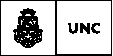
\includegraphics[width=5cm]{gfx/unc_logo} \\ \bigskip

        \vfill

        \LARGE

        \begingroup
            \color{CTtitle}\spacedallcaps{\myTitle} \\ \medskip
        \endgroup

        \LARGE

        \spacedlowsmallcaps{\myName} \\ \bigskip
        \spacedlowsmallcaps{Director:} \\
        \spacedlowsmallcaps{\mySupervisor} \\

        \vfill

        \Large

        \spacedlowsmallcaps{\myDegree} \\ \bigskip
        \myTime

        \vfill

    \end{center}

    \noindent\textit{\myTitle: \mySubtitle,} por \myName se distribuye bajo una \href{http://creativecommons.org/licenses/by-sa/4.0/}{Licencia Creative Commons Atribución-CompartirIgual 4.0 Internacional}. \vspace{0.3cm} \\
    \noindent\href{http://creativecommons.org/licenses/by-sa/4.0/}{
\includegraphics[width=2cm]{gfx/by-sa}}

    \vfill
  \end{addmargin}
\end{titlepage}

\thispagestyle{empty}

\hfill

\vfill

% \noindent\myName: \textit{\myTitle,} \mySubtitle, %\myDegree,
% \textcopyright\ \myTime

%\noindent\textit{\myTitle: \mySubtitle,} por \myName se distribuye bajo una \href{http://creativecommons.org/licenses/by-sa/4.0/}{Licencia Creative Commons Atribución-CompartirIgual 4.0 Internacional}. \vspace{0.3cm} \\
%\noindent\href{http://creativecommons.org/licenses/by-sa/4.0/}{
\includegraphics[width=2cm]{gfx/by-sa}}

%\bigskip
%
%\noindent\spacedlowsmallcaps{Supervisors}: \\
%\myProf \\
%\myOtherProf \\
%\mySupervisor
%
%\medskip
%
%\noindent\spacedlowsmallcaps{Location}: \\
%\myLocation
%
%\medskip
%
%\noindent\spacedlowsmallcaps{Time Frame}: \\
%\myTime

% \cleardoublepage%*******************************************************
% Dedication
%*******************************************************
\thispagestyle{empty}
\phantomsection
\pdfbookmark[1]{Dedication}{Dedication}

\vspace*{3cm}

\begin{center}
    \emph{Ohana} means family. \\
    Family means nobody gets left behind, or forgotten. \\ \medskip
    --- Lilo \& Stitch
\end{center}

\medskip

\begin{center}
    Dedicated to the loving memory of Rudolf Miede. \\ \smallskip
    1939\,--\,2005
\end{center}

%\cleardoublepage\include{FrontBackmatter/Foreword}
\cleardoublepage%*******************************************************
% Abstract
%*******************************************************
%\renewcommand{\abstractname}{Abstract}
\pdfbookmark[1]{Resumen}{Resumen}
% \addcontentsline{toc}{chapter}{\tocEntry{Abstract}}
\begingroup
\let\clearpage\relax
\let\cleardoublepage\relax
\let\cleardoublepage\relax

% I try to have four sentences in my abstract.
% The first states the problem.
% The second states why the problem is a problem.
% The third is my startling sentence.
% The fourth states the implication of my startling sentence.


\chapter*{Resumen}

Los meta-lenguajes de programación son una parte esencial de los asistentes de pruebas. Estos meta-lenguajes deben lidiar con multiples problemas y para esto utilizan diferentes mecanismos. En particular, el meta-lenguaje \Mtac en Coq utiliza mónadas como una forma de añadir tipado descriptivo a las tácticas de Coq.

Estos programas monádicos no son fáciles de desarrollar.
En parte, vincular cómputos monádicos puede ser una tarea complicada con el sistema de tipos de Coq, donde se utilizan tipos dependientes.
Solucionar estos problemas requiere de esfuerzo programacional inútil, no relacionado al objetivo.

Utilizando \mtac podemos crear un nuevo metaprograma que generalice la signatura de las funciones de forma casi automática, permitiendo una comunicación fluida entre declaraciones monádicas. % seamless interaction/communication

Con este trabajo, el programador puede concentrarse en lo verdaderamente importante y olvidarse de los detalles fuertemente restrictivos de la naturaleza de Coq, con un esfuerzo pequeño.

\chapter*{Abstract}

Meta-languages are an essential part of theorem provers. This meta-languages have to deal with several problems, hence they employ different mechanisms.
Particularly speaking, the meta-language \Mtac on Coq, utilizes monads as a means to add rich typed tactics to Coq.

This monadic programs are hard to develop. Partly, \textit{binding} monadic elements when Coq's type system uses dependent types is not simple.
Solving this involves great effort on developing useless code that is not related to the actual problem.

Using \Mtac we can create a new meta-program that can almost automatically generalize the signature of functions, allowing a seamless communication between monadic statements.

With this work, the programmer can focus on truly important tasks, forgetting the highly restrictable nature of Coq, with little effort.

\vfill

% \begin{otherlanguage}{ngerman}
% \pdfbookmark[1]{Zusammenfassung}{Zusammenfassung}
% \chapter*{Zusammenfassung}
% Kurze Zusammenfassung des Inhaltes in deutscher Sprache\dots
% \end{otherlanguage}

\endgroup

\vfill

%\cleardoublepage%*******************************************************
% Publications
%*******************************************************
\pdfbookmark[1]{Publications}{publications}
\chapter*{Publications}\graffito{This is just an early --~and currently ugly~-- test!}
This might come in handy for PhD theses: some ideas and figures have appeared previously in the following publications:

%\noindent Put your publications from the thesis here. The packages \texttt{multibib} or \texttt{bibtopic} etc. can be used to handle multiple different bibliographies in your document.

\begin{refsection}[ownpubs]
    \small
    \nocite{*} % is local to to the enclosing refsection
    \printbibliography[heading=none]
\end{refsection}

\emph{Attention}: This requires a separate run of \texttt{bibtex} for your \texttt{refsection}, \eg, \texttt{ClassicThesis1-blx} for this file. You might also use \texttt{biber} as the backend for \texttt{biblatex}. See also \url{http://tex.stackexchange.com/questions/128196/problem-with-refsection}.

%\cleardoublepage%*******************************************************
% Acknowledgments
%*******************************************************
\pdfbookmark[1]{Acknowledgments}{acknowledgments}

\begin{flushright}{\slshape
    We have seen that computer programming is an art, \\
    because it applies accumulated knowledge to the world, \\
    because it requires skill and ingenuity, and especially \\
    because it produces objects of beauty.} \\ \medskip
    --- \defcitealias{knuth:1974}{Donald E. Knuth}\citetalias{knuth:1974} \citep{knuth:1974}
\end{flushright}



\bigskip

\begingroup
\let\clearpage\relax
\let\cleardoublepage\relax
\let\cleardoublepage\relax
\chapter*{Acknowledgments}
Put your acknowledgments here.

Many thanks to everybody who already sent me a postcard!

Regarding the typography and other help, many thanks go to Marco
Kuhlmann, Philipp Lehman, Lothar Schlesier, Jim Young, Lorenzo
Pantieri and Enrico Gregorio\footnote{Members of GuIT (Gruppo
Italiano Utilizzatori di \TeX\ e \LaTeX )}, J\"org Sommer,
Joachim K\"ostler, Daniel Gottschlag, Denis Aydin, Paride
Legovini, Steffen Prochnow, Nicolas Repp, Hinrich Harms,
Roland Winkler, Jörg Weber, Henri Menke, Claus Lahiri,
Clemens Niederberger, Stefano Bragaglia, Jörn Hees,
Scott Lowe, Dave Howcroft, Jos\'e M. Alcaide, David Carlisle,
Ulrike Fischer, Hugues de Lassus, Csaba Hajdu, Dave Howcroft, 
and the whole \LaTeX-community for support, ideas and
some great software.

\bigskip

\noindent\emph{Regarding \mLyX}: The \mLyX\ port was intially done by
\emph{Nicholas Mariette} in March 2009 and continued by
\emph{Ivo Pletikosi\'c} in 2011. Thank you very much for your
work and for the contributions to the original style.


\endgroup

\cleardoublepage%*******************************************************
% Table of Contents
%*******************************************************
\pagestyle{scrheadings}
%\phantomsection
\pdfbookmark[1]{\contentsname}{tableofcontents}
\setcounter{tocdepth}{2} % <-- 2 includes up to subsections in the ToC
\setcounter{secnumdepth}{3} % <-- 3 numbers up to subsubsections
\manualmark
\markboth{\spacedlowsmallcaps{\contentsname}}{\spacedlowsmallcaps{\contentsname}}
\tableofcontents
\automark[section]{chapter}
\renewcommand{\chaptermark}[1]{\markboth{\spacedlowsmallcaps{#1}}{\spacedlowsmallcaps{#1}}}
\renewcommand{\sectionmark}[1]{\markright{\textsc{\thesection}\enspace\spacedlowsmallcaps{#1}}}
%*******************************************************
% List of Figures and of the Tables
%*******************************************************
\clearpage
% \pagestyle{empty} % Uncomment this line if your lists should not have any headlines with section name and page number
\begingroup
    \let\clearpage\relax
    \let\cleardoublepage\relax
    %*******************************************************
    % List of Figures
    %*******************************************************
    %\phantomsection
    %\addcontentsline{toc}{chapter}{\listfigurename}
    \pdfbookmark[1]{\listfigurename}{lof}
    \listoffigures

    \vspace{8ex}

    %*******************************************************
    % List of Tables
    %*******************************************************
    %\phantomsection
    %\addcontentsline{toc}{chapter}{\listtablename}
    \pdfbookmark[1]{\listtablename}{lot}
    \listoftables

    \vspace{8ex}
    % \newpage

    %*******************************************************
    % List of Listings
    %*******************************************************
    %\phantomsection
    %\addcontentsline{toc}{chapter}{\lstlistlistingname}
    \pdfbookmark[1]{\lstlistlistingname}{lol}
    \lstlistoflistings

    \vspace{8ex}

    %*******************************************************
    % Acronyms
    %*******************************************************
    %\phantomsection
    \pdfbookmark[1]{Acronyms}{acronyms}
    \markboth{\spacedlowsmallcaps{Acronyms}}{\spacedlowsmallcaps{Acronyms}}
    \chapter*{Acronyms}
    \begin{acronym}[UMLX]
        \acro{DRY}{Don't Repeat Yourself}
        \acro{API}{Application Programming Interface}
        \acro{UML}{Unified Modeling Language}
    \end{acronym}

\endgroup


%********************************************************************
% Mainmatter
%*******************************************************
\cleardoublepage
\pagestyle{scrheadings}
\pagenumbering{arabic}
%\setcounter{page}{90}
% use \cleardoublepage here to avoid problems with pdfbookmark
\cleardoublepage
%************************************************
\part{Introducción}\label{pt:introduccion}
\section{Introducción}
\section{Coq}

En este capitulo introduciremos las características más relevantes del asistente de pruebas interactivo Coq. El objetivo de este capitulo es introducir todos los conceptos que utilizaremos más adelante, pero esto significa que no es una introducción completa.

El desarrollo de Coq comenzó en 1984 con el apoyo de INRIA como el trabajo de Gérard Huet y Thierry Coquand. En ese momento Coquand estaba implementado un lenguaje llamado \textit{Calculus of Constructions} cuando el 1991 una nueva implementación basada en un Calculus of Inductive Constructions extendido comenzó a ser desarrollado tomando el nombre de Coq.

Ahora mismo Coq es desarrollado por más de 40 desarrolladores activos y es reconocido como unos de los asistentes de prueba principales.

Como un asistente de pruebas la orientación de Coq es la de permitir la escritura totalmente formal de teoremas y pruebas, y asegurarnos de su correción. Se parte de lo que se denomina \textit{kernel}, el nucleo de Coq, que es el que verifica que la prueba corresponde al teorema, es decir, que sea correcta. De esta forma, el humano no está encargado de verificar la prueba, solo de escribirla.
% TODO: diferencia con otros asistentes

\subsection{Los lenguajes Coq}

Coq no es técnicamente un lenguaje de programación, si no un asistente de pruebas. Pero podemos encontrar múltiples lenguajes dentro de Coq que nos permiten expresarnos. 
\begin{itemize}
    % TODO: cita Gallina? http://adam.chlipala.net/cpdt/html/Universes.html
    \item \textit{Gallina}: este es el lenguaje de especificación de Coq. Permite desarrollar teorías matemáticas y probar especificaciones de programas. Utilizaremos extensivamente un lenguaje muy similar a este para definir nuestros programas en Mtac2.
    % TODO: cita Ltac?
    \item \textit{Ltac}: este el lenguaje en que se definen las \textit{tácticas} de Coq. Dado que Coq está centrado en las tácticas, Ltac es una de las partes centrales del aparato.
    \item \textit{Vernacular}.
\end{itemize}

Aunque Coq no es un lenguaje de programación propiamente dicho, este puede ser utilizado como un lenguaje de programación funcional. Estos programas serán especificados en Gallina. Dada la naturaleza de Coq como provador de teoremas, estos programas son funciones puras, es decir, no producen efectos secundarios y siempre terminan.

\subsection{La teoría de Coq}

\textit{Calculus of Inductive Constructions} es la base de Coq. Este es un cálculo lambda tipado de alto orden y puede ser interpretado como una extensión de la correspendencia Curry-Howard.

Llamaremos \textit{Terms} (o términos) a los elementos básicos de esta teoría. Terms incluye \textit{Type}, \textit{Prop}, variables, tuplas, funciones, entre otros. Estás son algúnas de las herramientas que utilizaremos para escribir nuestros programas.

% TODO: Ampliar sobre las capacidades de Coq.

\subsection{Tipos de datos y Funciones}

Ahora aprenderemos a codificar nuestros programas funcionales en Coq. Lo primero que debemos entender es que operamos sobre \textit{términos} y algo es un término si tiene tipo. Coq provee muchos tipos predefinidos, por ejemplo \lstinline{unit}, \lstinline{bool}, \lstinline{nat}, \lstinline{list}, entre otros. A continuación estudiaremos cómo definir tipos y funciones.

Veamos cómo se define el tipo \lstinline{bool}:
\begin{lstlisting}
Inductive bool : Set :=
  | true : bool
  | false : bool.
\end{lstlisting}
Como podemos observar, es un tipo inductivo, especificado por la keyword \lstinline{Inductive}, con dos constructores \lstinline{true} y \lstinline{false}. De por sí, el tipo \lstinline{bool} no posee un significado hasta que nosotros lo proveamos de uno. Podemos ahora intentar definir algunos operadores booleanos.
\begin{lstlisting}
Definition andb (b1 b2:bool) : bool := if b1 then b2 else false.
Definition orb (b1 b2:bool) : bool := if b1 then true else b2.
Definition implb (b1 b2:bool) : bool := if b1 then b2 else true.
Definition negb (b:bool) := if b then false else true.
\end{lstlisting}
Las definiciones de funciones no recursivas comienzan con el keyword \lstinline{Definition}. La primera se llama \lstinline{andb} y toma dos booleanos como argumentos y retorna un booleano. Se utiliza la notación \lstinline{if b then x else y} para matchear sobre los booleanos de manera más fácil. Finalmente podemos definir una función más interesante.
\begin{lstlisting}
Definition Is_true (b:bool) :=
  match b with
    | true => True
    | false => False
  end.
\end{lstlisting}

Ahora, veamos un tipo con un ingrediente un poco más complicado, \lstinline{nat}.
\begin{lstlisting}
Inductive nat : Set :=
  | O : nat
  | S : nat -> nat.
\end{lstlisting}
Notemos que el constructor \lstinline{S} es una función que recibe un término de tipo {nat}, es decir, \lstinline{nat} es un tipo recursivo. Por ejemplo el término \lstinline{S (S O)} es de tipo \lstinline{nat} y representa al número 2.

Para continuar con este desarrollo, veamos el tipo de \lstinline{list} que es polimórfico.
\begin{lstlisting}
Inductive list (A : Type) : Type :=
  | nil : list A
  | cons : A -> list A -> list .
\end{lstlisting}
Este tipo es un tipo polimórfico dado que requiere de un \lstinline{A : Type}. Por ejemplo, una posible lista es \lstinline{cons (S O) nil : list nat} que representa a la lista con un único elemento 1 de tipo \lstinline{nat}.

Definiremos una función que añade un elemento a una lista.
\begin{lstlisting}
Definition add_list {A} (x : A) (l : list A) : list A :=
  cons x l.
\end{lstlisting}
Dado que el tipo \lstinline{A} puede ser inferido facilmente por Coq, utilizamos llaves a su alrededor para expresar que sea un argumento implícito. En el cuerpo de la función solo utilizamos \lstinline{cons}, uno de los constructores de \lstinline{list}, para añadir un elemento delante de \lstinline{l}.

Ahora nos interesa definir la función \lstinline{length} que retorna el largo de una lista.
\begin{lstlisting}
Fixpoint len {A} (l : list A) : nat :=
match l with
| [] => O
| x :: xs => S (len xs)
end.
\end{lstlisting}
Coq está diseñado de forma que necesitamos utilizar el keyword \lstinline{Fixpoint} para poder definir funciones recursiva. Aquí Coq está encontrando el argumento decreciente de la función \lstinline{len} y por eso acepta nuestra definición. El cuerpo de \lstinline{len} inspecciona a \lstinline{l} y lo \textit{matchea} con el caso correspondiente. Utilizamos \lstinline{S} y \lstinline{O}, los constructores de \lstinline{nat} para expresar el valor de retorno.

\subsection{Tipos dependientes}

Una de las herramientas más importantes que hay en Coq son los tipos dependientes. Estos nos permiten hablar de elementos que dependen de otros anteriores. Por ejemplo, puede ser de nuestro interés hablar de números positivos, en otras palabras, \lstinline{x : nat} tal que \lstinline{x <> O}. En este caso, \lstinline{x <> O} es una prueba que depende de \lstinline{x} y solo existirá cuando \lstinline{x} sea mayor a 0.

Para hablar de un ejemplo práctico de tipos dependientes, hemos elegido la función \lstinline{head} que retorna la cabeza de una lista. Comencemos con la versión más simple, donde utilizamos un valor default \lstinline{d} para el caso en que la lista es vacía.
\begin{lstlisting}
Definition head_d {A} (l : list A) (d : A) : A :=
  match l with
  | [] => d
  | x :: xs => x
  end.
\end{lstlisting}
El problema de esta solución es que a excepción de que \lstinline{d} sea un valor único, no hay manera de saber si la función retornó realmente la cabeza de la lista.

La segunda opción es utilizar el tipo \lstinline{option}.
\begin{lstlisting}
Inductive option A : Type :=
| None : option A
| Some : A -> option A.
\end{lstlisting}
Con este tipo auxiliar podemos reescribir \lstinline{hd}.
\begin{lstlisting}
Definition head_o {A} (l : list A) : option A :=
  match l with
  | [] => None
  | x :: xs => Some x
  end.
\end{lstlisting}
Esta solución es mejor que la anterior pero sigue sufriendo de una deficiencia. Dado que \lstinline{head_o} retorna un \lstinline{option} no sabemos si el resultado de esta función será realmente un elemento o si será el constructor vacío, por lo que todas las funciones que utilicen a \lstinline{head_o} deben también utilizar \lstinline{option}.
% TODO: citar? failure is not an option

Esto nos lleva a nuestra última solución. Esta requiere que nos aseguremos que la lista \lstinline{l} no es vacia, es decir, \lstinline{l <> []}. Pero para entenderla debemos ver dos cosas más: $\Sigma$\textit{-types} y \lstinline{Program}.
% TODO: sigma types.
Intuitivamente, los $\Sigma$\textit{-types} son tuplas donde el argumento de la derecha es dependiente del de la izquierda. A continuación, la definición.
\begin{lstlisting}
Inductive sig (A : Type) (P : A -> Prop) : Type :=
  exist : \forall x : A, P x -> {x : A | P x}
\end{lstlisting}
Se utiliza la notación \lstinline|{x : A \| P x}| para expresar \lstinline{sig A (fun x => P)}.
% TODO: está bien la notación?

\lstinline{Program} es una libreria que permite progamar en Coq como si fuera un lenguaje de programación funcional mientras que se utiliza una especificación tan rica como se desee y probando que el codigo cumple la especificación utilizando todo el mecanizmo de Coq. En nuestro caso utilizaremos \lstinline{Program} para codificar \lstinline{head} de una manera casi transparente.
\begin{lstlisting}
Program Definition head {A}
(l : list A | [] <> l ) : A :=
  match l with
  | [] => !
  | x :: xs => x
  end.
\end{lstlisting}
Como podemos observar, la única diferencia es que la signatura de \lstinline{head} especificamos que \lstinline{l} es una lista junto con una prueba que muestra que no es vacía.

\subsection{Tácticas}

En la próxima sección hablaremos de pruebas, metas (\textit{goals}) y tácticas. Para esto introduciremos un ejemplo que nos facilite entender estos conceptos.

\begin{exmp}\label{exmp:sub_0_r}
\begin{lstlisting}
Lemma sub_0_r : forall n, n - 0 = n.
Proof. intro n. case n; [ | intro n']; reflexivity. Qed. 
\end{lstlisting}
\end{exmp}

% TODO: cita Ltac https://coq.inria.fr/refman/zebibliography.html#del00
% TODO: Utilizar tácticas de Coq. Mencionar que hay múltiples librerías de tacticas.

El teorema a probar restar 0 a cualquier número $n$ es $n$. Ya que la resta está definida por pattern matching en el primer argumento, esta igualdad no es automáticamente cierta computando. Por eso, debemos hacer análisis por casos.

El código comienza con el comando \lstinline{Lemma}, donde efectivamente definimos lo que queremos probar.
Luego utilizamos el comando \lstinline{Proof} para indicar el inicio de la prueba, la cual será resuelta a través de la concatenación de tácticas de Ltac. Estas tácticas trasnforman el \textit{proof-state} incrementalmente construyendo un \textit{proof-term}, la prueba.

Después de \lstinline{Proof}, Coq genera una \lstinline{goal}, una meta. Internamente, una meta en Coq es representada con una \textit{meta-variable}. Esta meta-variable tiene un tipo, en concreto el lema que queremos probar. En este caso nuestra meta $?g$ tiene tipo \lstinline{\forall n, n - 0 = n}.

Para introducir la variable $n$, utilizamos \lstinline{intro}. Esta instancia a $?g$ como \lstinline{fun n:nat => $?g_1$} donde el tipo de $?g_1$ es \lstinline{n - 0 = n}.

% TODO: Contextual Modal Type Theory, Nanevsky 2008.
Ya introducida la variable, el próximo paso es hacer análisis por casos en ella. Con \lstinline{case} podemos analizar a $n$ según los constructores de su tipo. Para el primer caso: \lstinline{0 - 0 = 0} es trivial. El segundo caso es \lstinline{\forall n':nat, S n' - 0 = S n'}, para el cual, primero introduciremos $n'$ y luego, por la naturaleza inductiva de la resta, será igualmente trivial para Coq. La táctica \lstinline{case} retorna estas dos sub-metas, las cuales componemos, con el operador de composición (el punto y coma), con las tácticas listadas en \lstinline{[ | intro n']}. La primer sub-meta es resuelta por la táctica a la izquierda del \lstinline{|}, que es implicitamente la táctica identidad (\lstinline{idtac}), mientras que la segunda sub-meta es resuelta por la táctica a la derecha de \lstinline{|}, \lstinline{intro n'}. La salida de esta composición son de nuevo dos tácticas las que de nuevo compondremos con \lstinline{reflexivity}. Esto signfica que aplicaremos \lstinline{reflexivity} a ambas tácticas resultantes, resolviendolas trivialmente por computación.

\subsection{Interfaz interactiva}

Cuando se dice que Coq es un asistente \textit{interactivo} nos referimos a que Coq nos puede ayudar a desarrollar la prueba en cierta medida.
% TODO: UI de Coq, dar ejemplos.
Por ejemplo, supongamos que queremos probar el siguiente teorema.
\begin{exmp}
\begin{lstlisting}
Definition le_S (n : nat) : n <= S n.
\end{lstlisting}
\end{exmp}
Al entrar a alguno de los editores de textos compatibles con Coq (Emacs, Visual Studio Code o CoqIDE) cargamos el teorema y Coq entrará al modo interactivo, en el cual nos mostrará el estado actual de la prueba. En este caso comenzamos con la hipótesis \lstinline{n : \nat} ya en nuestro contexto y una única meta $?g$ de tipo \lstinline{n <= S n}. Ahora aplicamos inducción en \lstinline{n} obteniendo dos sub-metas: $?g_1$ con tipo \lstinline{0 <= S 0} y $?g_2$ con tipo \lstinline{S n <= S (S n)}. Para la primera meta $?g_1$ utilizamos \lstinline{apply} para aplicar el teorema \lstinline{le_0_n} instanciado con \lstinline{S n}, esto soluciona automaticamente la sub-meta. La segunda sub-meta se resuelve de una manera similar, solo que tenemos una hipótesis inductiva \lstinline{IHn}.

En la figura \ref{fig:ui} podemos observar como se nos presenta esta información.

\begin{figure}[h]
  \centering
  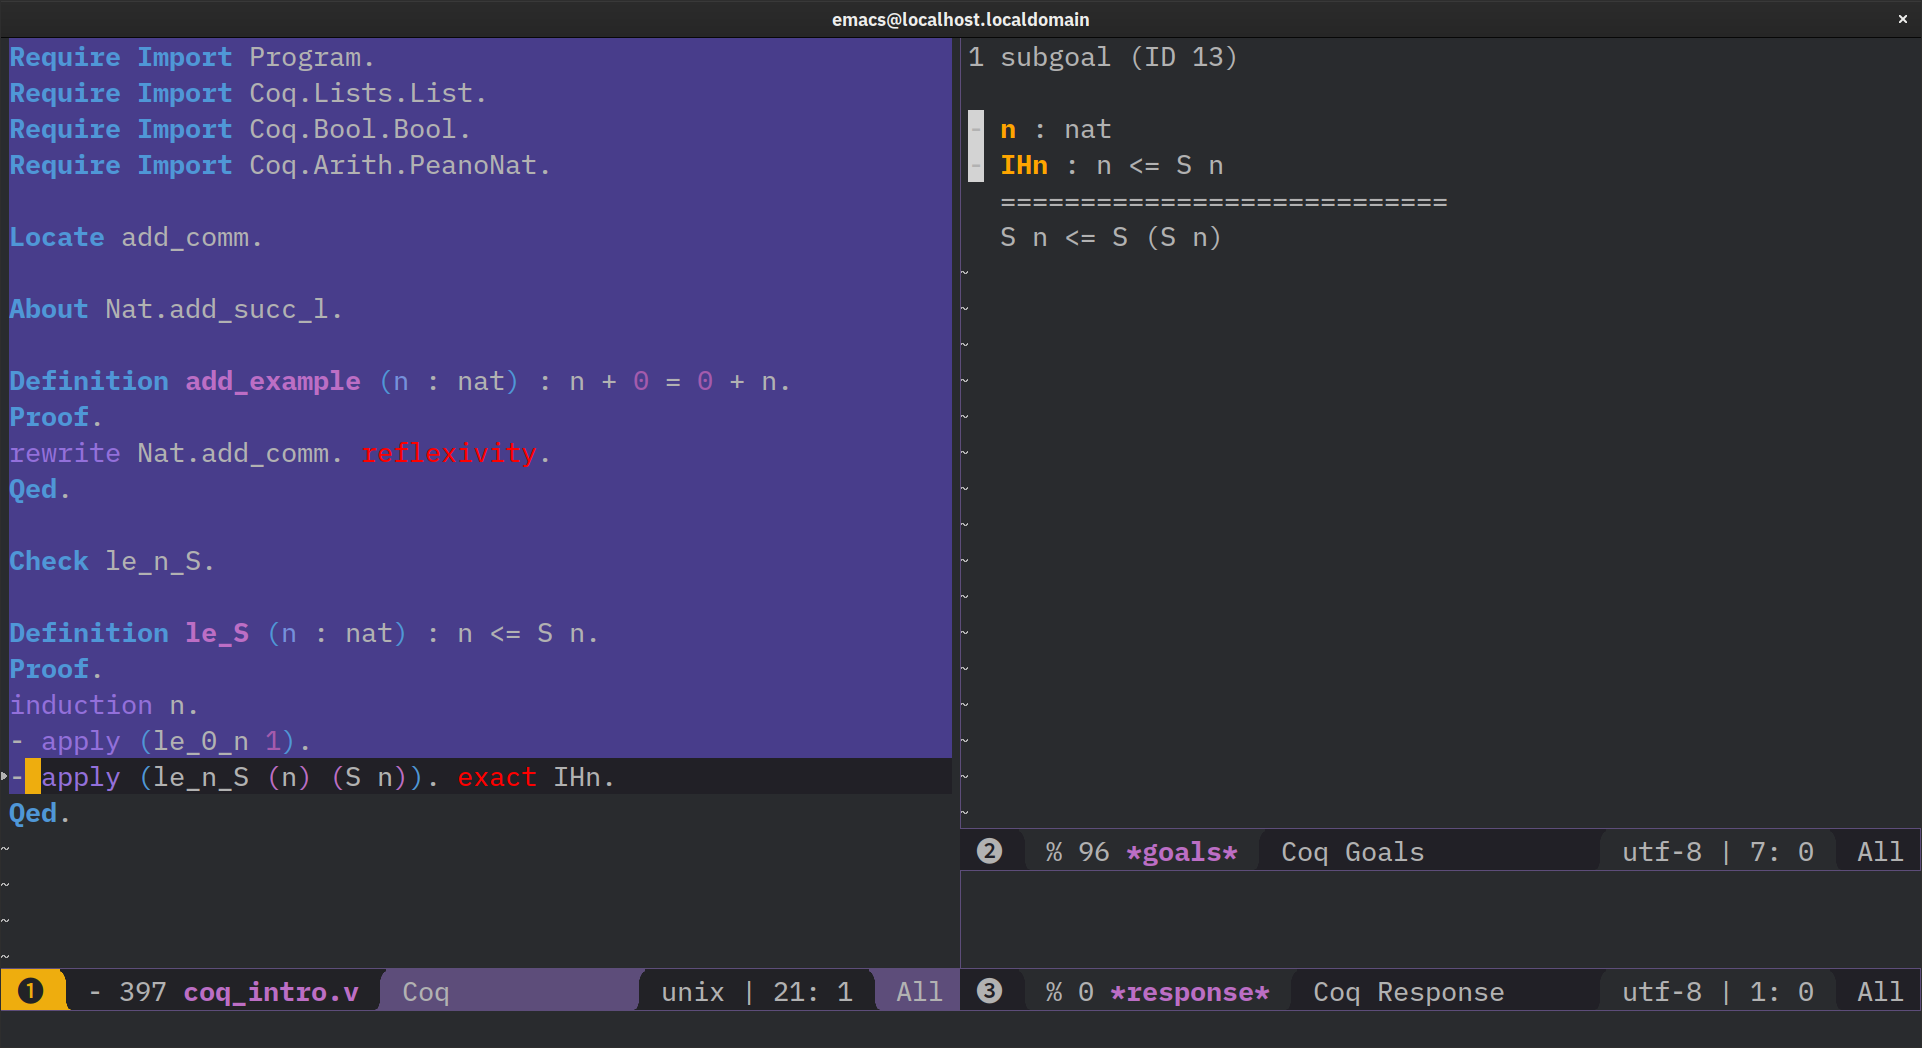
\includegraphics[width=1\textwidth]{gfx/coq_emacs_example.png}
  \caption{Ejemplo de interfaz de Coq}
  \label{fig:ui}
\end{figure}

Coq cuenta con muchos comandos que se usan constantemente.
\begin{itemize}
  \item \lstinline{Check} imprime el tipo de un término. Cuando es llamado en modo prueba, el término es chequeado en el contexto local de la sub-meta.
  \item El comando \lstinline{About} muestra información general.
  \item \lstinline{Print}:
  \item \lstinline{Locate}:
  \item \lstinline{Eval}:
\end{itemize}
\chapter{Mtac2}\label{ch:mtac2}

\Mtac \cite{DBLP:journals/pacmpl/KaiserZKRD18} es un metalenguaje de programación para Coq. Esto quiere decir que complementa a Coq, permitiendo ``hacer Coq'' de una manera distinta. En el trabajo, nos centramos en ampliar \Mtac y por eso es importante que veamos que nos permite hacer y cómo.

\section{Mónadas}

Las mónadas son uno los métodos que utilizan los lenguajes de programación funcional para la representación de efectos secundarios.
\Mtac define una mónada que es la que permite añadir una serie de características muy útiles a la hora de desarrollar metaprogramas.
Las tácticas presentes en \mtac son metaprogramas monádicos.

Utilizamos la función \lstinline{M : Type -> Prop} para referirnos a la versión monádica de un tipo cualquiera. A partir de los tipos monádicos, pasamos a tener elementos monádicos. Estos elementos reflejan pasos computacionales y se construyen a través de dos funciones: \lstinline{bind} compone pasos computacionales, y \lstinline{return} o \lstinline{ret} los envuelve en la mónada. Por ejemplo, podemos tener el tipo \lstinline{M nat} que expresa posibles valores de números naturales. La expresión \lstinline{ret 5} expresa un valor de \lstinline{M nat}.

\section{Confección de Metaprogramas}

% Ya habiendo mencionado tácticas, tornaremos nuestra atención a meta-programas.
Las tácticas de \mtac son metaprogramas.
Estos programas se caracterizan por ser monádicos, es decir, utilizan mónadas para reflejar efectos secundarios.
Esto se amplía a muchas características útiles, pero nada es gratis.
A continuación intentaremos comprender las limitaciones impuestas por el metalenguaje.

Comenzaremos analizando \lstinline{mmatch}. Como ya vimos en Gallina, \lstinline{match} es puro, o sea, cuando lo utilizamos, necesitamos matchear todos los casos del constructor y a su vez no podemos matchear en términos que no sean constructores del tipo.
Mientras tanto, \lstinline{mmatch} nos permite matchear más libremente.
Esto significa que podemos matchear en expresiones sintácticas de manera de separarlas muy específicamente para nuestra conveniencia.
Un ejemplo puede ser el siguiente.
Imaginemos un programa que a todo número le suma uno, pero específicamente no modifica el número original si este está expresado como una suma. Esto se puede expresar de la siguiente forma en \Mtac.

\begin{lstlisting}
Definition test_match (n : nat) : M nat :=
  mmatch n with
  | [? x y] add x y => ret n
  | O => ret (S O)
  | [? n'] S n' => ret (S (S n'))
  end.
\end{lstlisting}

El único detalle extraño que podemos encontrar es que en dos de los casos tenemos unos corchetes antes de la expresión.
Esto se utiliza para decirle a \Mtac que estas variables están siendo introducidas al contexto.

Para hacer programas recursivos utilizaremos \lstinline{mfix}. Existen múltiples variantes para una cantidad distinta de argumentos recursivos: \lstinline{mfix1}, \lstinline{mfix2}, etcetera.

Un ejemplo puede ser el de \lstinline{map}.

\begin{lstlisting}
Definition map {A} {B} (t : A -> B) : \forall (l : list A), M (list B) :=
mfix1 m (l : list A) : M list B :=
  mmatch l with
  | nil => ret nil
  | [? x xs] x::xs => xs' <- m xs;
                            ret ((t x)::xs')
  end.
\end{lstlisting}

En \lstinline{map} solo tenemos un argumento recursivo, que será la lista que estamos mapeando.
En el ejemplo también vemos el uso de la notación \lstinline{<-}.
Esta indica que estamos \emph{bindeando} a la variable \lstinline{xs'} con el cómputo \lstinline{m xs}, es decir, utilizando la función \lstinline{bind} para conectar estos cómputos.
En otros ejemplos es posible que veamos otra notación: \lstinline{;;}.
Está notación también indica el uso de \lstinline{bind}, con la diferencia de que no nos interesa el valor que estamos vinculando.
Usualmente lo observaremos al utilizar la función \lstinline{print}, ya que esta función retorna un argumento de tipo \lstinline{M unit}.

Los últimos dos elementos que necesitamos entender son \lstinline{mtmmatch} y \lstinline{mfix}.
Estas son versiones de \lstinline{mmatch} y \lstinline{mfix$_n$}, respectivamente.

En primer lugar, utilizaremos \lstinline{mtmmatch} para realizar pattern matching monádico, con la diferencia de que los valores de retorno pueden ser dependientes, es decir, podemos retornar funciones que computan mónadas.

Por último, \lstinline{mfix} es una versión general de la recursión monádica, esta puede tomar una cantidad arbitraria de argumentos. Está motivada por la limitación de \lstinline{mfix1}, \lstinline{mfix2} y \lstinline{mfix3}.
Aún así, su uso no es estándar porque todavía está en desarrollo.

\section{El costo de la mónada}

Como mencionamos anteriormente, las funcionalidades de \Mtac tienen un coste.
Imaginemos que estamos calculando el cociente entre dos números enteros, siendo el divisor igual a cero.
Entonces el programa no puede calcular el cociente y debe fallar.
Esto nos muestra la gran diferencia entre un programa de Coq y uno de \mtac: un programa monádico puede fallar.
Mientras tanto, en el mundo de Coq este concepto no existe.
Un programa que retorna un número entero, debe retornar un entero, y más aún, un programa que tiene el tipo de una proposición, efectivamente es una prueba de la misma.
Supongamos esa proposición es \lstinline{P : Prop}.
Ahora para probarla monádicamente necesitamos un programa \lstinline{p : M P}, pero para cualquier \lstinline{P} podemos escribir dar un programa con esa signatura y que no sea una prueba.

\begin{lstlisting}
Definition univ (P : Prop): M P :=
  raise MyException.
\end{lstlisting}

Con \lstinline{raise} podemos levantar una excepción, en esta caso \lstinline{MyException} es una excepción definida por nosotros.
Sin la presencia de la mónada esto no sería posible.
La mónada nos quita garantías que, si no, tendríamos en Coq.

Dada esta limitación todas las funciones nativas de Coq pueden ser utilizadas en los tipos de las funciones, pero no sucede lo mismo con las funciones monádicas.
Esto hace que el desarrollo de metaprogramas se tenga que pensar de manera estratégica: qué funciones serán monádicas y cuales serán nativas de Coq.

\section{Alternativas}
% TODO: referencias https://popl19.sigplan.org/details/CoqPL-2019/8/Ltac2-Tactical-Warfare

\Mtac no es el único metalenguaje de programación para Coq. 

\graffito{TODO: cita de Ltac2}
Un ejemplo de otro metalenguaje es \emph{Ltac2}.
Este funciona como un \emph{wrapper} alrededor del \emph{proof engine} de Coq.
Implementa una $\alpha$ táctica de tipo monádico en OCaml y trata de conservar la mayor parte de Ltac posible, busca la mayor retrocompatibilidad.

Otras alternativas pueden ser Template-Coq \cite{DBLP:conf/itp/AnandBCST18}, Rtac \cite{DBLP:conf/esop/MalechaB16} y Coq-Elpi \cite{tassi:hal-01637063}.

La gran diferencia entre estos metalenguajes es que \Mtac es \emph{shallowly embedded}, mientras que los otros no. A diferencia de \Mtac, los objetos de estas alternativas son términos de un tipo inductivo \lstinline{Term}, es decir, no tienen un tipo informativo. Es decir, en \Mtac un programa \lstinline{M A} está garantizado que, si termina correctamente, retorna un término de tipo \lstinline{A}. Pero en los lenguajes \emph{deeply embedded}, como los mencionados, nada garantiza que el término retornado tenga un tipo dado, puede retornarse cualquier elemento de cualquier tipo, incluso términos mal construidos.

\section{Telescopios}

Los \emph{telescopios} son una estructura de datos inductiva de \Mtac que permite expresar una secuencia de tipos o valores, posiblemente dependientes, y de largo arbitrario.
Los telescopios, junto con las funciones que lo acompañan, serán claves a la hora de poder expresar nuestro problema y consecuente solución.

\begin{lstlisting}[float=h,frame=tb,caption={Definicion de telescopio},label=lst:MTele]
Inductive MTele : Type :=
| mBase : MTele
| mTele {X : Type} (F : X -> MTele) : MTele.
\end{lstlisting}

El tipo \lstinline{MTele} crea una cadena de abstracciones.
Este se codifica a través de funciones, lo que permite que sean dependientes, es decir, un telescopio puede tener elementos que dependan de elementos anteriores.

Definiremos la siguiente notación para poder referirnos a los telescopios de una manera más accesible.

El constructor \lstinline{mBase} representa el telescopio vacío o de largo cero. Representaremos con \lstinline{[$\;$]$_t$} a \lstinline{mBase}.

Para un telescopio de largo $n$, tenemos al constructor \lstinline{mTele} anidado $n$ veces. Dado que podemos pensar al telescopio como una secuencia dependiente de tipos, un posible comienzo es \lstinline{[T$_0$ : Type ;> ...]$_t$}. Ahora, todos argumentos siguientes del telescopio pueden depender de \lstinline{T$_0$}. Luego, \lstinline{[T$_0$ : Type ;> T$_1$ : T$_0$ -> Type ;> ...]$_t$} tiene sentido, y el tipo \lstinline{T$_1$} depende de \lstinline{T$_0$}. Tranquilamente se puede dar el caso es que ningún argumento dependa de \lstinline{T$_0$}.

\begin{lstlisting}[frame=tb,caption={Notación de telescopios},label=lst:not_tele]
(* ej 1 *) mBase $\equiv$ [$\;$]$_t$
(* ej 2 *) mTele (fun T : Type => mTele R : T -> Type) $\equiv$
[T : Type ;> R : (T -> Type)]$_t$
(* ej 3 *) mTele (fun T : Type => mTele t : T) $\equiv$
[T : Type ;> t : T]$_t$
\end{lstlisting}

Para comenzar a estudiar a este tipo, podemos pensar que existen jerarquías.
La primera jerarquía sería la de los telescopios en sí, elementos de tipo \lstinline{MTele}.
Ahora, dado un \lstinline{m : MTele}, la segunda jerarquía es la de los tipos generados por el telescopio \lstinline{m}.
Luego, el último nivel es el de los elementos de este nuevo tipo telescopico.

Veremos esto en mayor profundidad, pero para eso debemos primero definir el tipo \lstinline{Sort}.

\begin{lstlisting}[frame=tb,caption={Definición de \lstinline{Sort}},label=lst:Sort]
Inductive Sort : Type := \Prop_sort | \Type_sort.
\end{lstlisting}

Dentro de unos párrafos, utilizaremos \lstinline{Sort} para abstraer el concepto de tipo y proposición, y poder aplicar ciertas funciones telescópicas.

\begin{itemize}
  \item En el nivel superior, definimos nuestro telescopio \lstinline{m} de largo $n$ con dependencias arbitrarias. Esto es simplemente utilizando los constructores de \lstinline{MTele}.
  \item Ya con \lstinline{m} definido, podemos utilizar la función \lstinline{MTele_Sort} para computar un tipo derivado del telescopio. Sea \lstinline{(s : Sort)}, es decir, \lstinline{s} es \lstinline{\Type_sort} o \lstinline{\Prop_sort}, la expresión \lstinline{(MTele_Sort s m)} es un tipo, y específicamente, es el tipo \lstinline{\forall x$_1$ x$_2$ ... x$_n$, s}.
  \item Como dijimos, \lstinline{(MTele_Sort s m)} es un tipo, por lo tanto, podemos tener elementos de ese tipo. Esta sería la última jerarquía.
  
  Para esto utilizamos la función \lstinline{MTele_val}. Esta función toma un valor de \lstinline{(MTele_Sort s m)} y retorna un valor de tipo \lstinline{s}. Por cómo es el tipo, esto signfica que un valor del mismo es algo de la forma \lstinline{(fun x$_1$ x$_2$ ... x$_n$ => T x$_1$ x$_2$ ... x$_n$)} para algún \lstinline{T}. Luego, \lstinline{MTele_val} retornará un valor de tipo \lstinline{s}, es decir, \lstinline{T y$_1$ y$_2$ ... y$_n$} para algunos \lstinline{y$_i$}.
\end{itemize}

Utilizaremos \lstinline{MTele_Ty} y \lstinline{MTele_Prop} para expresar \lstinline{MTele_Sort \Type_sort} y \lstinline{MTele_Sort \Prop_sort} respectivamente.

\subsection{Funciones extra}

Los telescopios de \Mtac traen consigo muchas funciones que son las que le dan el poder expresivo que los hace útiles. 

La función \lstinline{MTele_C} permite mapear a un \lstinline{MTele_Sort} con una función constante.
Por ejemplo, la mónada que hemos observado antes: \lstinline{M}, en realidad es una función de \lstinline{Type} en \lstinline{Prop}.
Entonces podríamos tomar un tipo \lstinline{\forall x$_1$ ... x$_n$, T x$_1$ ... x$_n$} y transformalo en \lstinline{\forall x$_1$ ... x$_n$, M (T x$_1$ ... x$_n$)}

\graffito{TODO: Agrego más?}
Con \lstinline{MTele_In} podemos ganar acceso a múltiples tipos y valores telescopios al mismo tiempo, así siendo capaces de computar un nuevo tipo telescópico.
Al momento de utilizarlo lo estudiaremos en más profundidad.

\subsection{Ejemplo}

Para que los conceptos queden claros vamos a plantear un ejemplo de telescopios.

Primero definimos un telescopio \lstinline{m}.

\begin{lstlisting}
Definition m := [T : Type ;> l : list T ;> p : length l = 0]$_t$
\end{lstlisting}

Si ahora inspeccionamos quien es \lstinline{MTele_Sort \Type_sort m} veremos que es lo esperado.

\begin{lstlisting}
Eval cbn in MTele_Ty m.
= \forall (T : Type) (l : list T), length l = 0 -> Type : Type
\end{lstlisting}

El próximo paso es hablar de elementos de este tipo.

\begin{lstlisting}
Definition Tm : MTele_Ty m := fun T l p => l = nil.
\end{lstlisting}

Donde tenemos \lstinline{l <> nil} podemos poner cualquier tipo.
Podriamos tener \lstinline{nat}, pero para hacerlo más interesante definimos un tipo con sentido.
Lo importante es que Coq acepta la definición de \lstinline{Tm}, lo que implica que esta definición efectivamente tiene tipo el tipo esperado.
Si este no fuera el caso, el type-checker de Coq no lo aceptaría.
El próximo paso es definir un elemento del tipo \lstinline{Tm}.

Podemos definir el siguiente teorema y probarlo.

\begin{lstlisting}
Definition test_Tm : forall T (l : list T) (p : List.length l = 0), l = nil.
intros T l p. by apply length_zero_iff_nil.
Qed.
\end{lstlisting}

El truco es que al conocer a \lstinline{Tm} sabemos que esta función tiene ese tipo.
Finalmente, podemos definir lo siguiente.

\begin{lstlisting}
Definition vm : MTele_val tm := test_Tm.
\end{lstlisting}

Efectivamente, \lstinline{test_Tm} tiene tipo \lstinline{MTele_val tm}.

% % En este archivo definimos la verdadera salsa!
\section{Telescopios}

En Mtac2 llamamos \textit{telescopios} a una estructura de datos inductiva
que permite expresar una cantidad arbitraria de tipos.

\begin{lstlisting}
Inductive MTele : Type :=
| mBase : MTele
| mTele {X : Type} (F : X -> MTele) : MTele.
\end{lstlisting}

El tipo \lstinline{MTele} crea una cadena de abstracciones que toma valores de tipos específicos.

Los telescopios, junto con las funciones que lo acompañan será la base para nuestro
trabajo.

Eeste tipo puede pensarse en varias jerarquías.
La primera sería el telescopio mismo.
Un ejemplo puede ser:

\begin{lstlisting}
Let m := @mTele nat (fun _ : nat => mBase)
\end{lstlisting}

Este telescopio lleva un único tipo, \lstinline{nat}.
Luego existen una infinita cantidad de tipos que dependen de \lstinline{m}, para
continuar el ejemplo elegimos uno.

\begin{lstlisting}
Let A : MTele_Sort SProp m := fun x => x = x.
\end{lstlisting}

Finalmente, nos interesa un valor de ese tipo, es decir, una prueba.

\begin{lstlisting}
Let a : MTele_val (MTele_C SProp SProp M A) := fun x => ret (eq_refl).
\end{lstlisting}
 Unido a mtac2
\cleardoublepage
%************************************************
% \ctparttext{You can put some informational part preamble text here.}
\part{Lift}\label{pt:lift}
\chapter{Motivación}\label{ch:motivacion}

% Se asume que se explicó que es Mtac2 en la introducción y todas las cosas que
% se pueden hacer.
\textsc{Mtac2} nos permite definir funciones monádicas. Estas cuentan con ciertas ventajas.
La siguiente función calcula el máximo de una lista de números \lstinline{nat : Set} y utiliza \lstinline{mtmmatch} para hacer un análisis sintáctico, a diferencia de \lstinline{match}.

\begin{lstlisting}[frame=tb,caption={Función \lstinline{list_max_nat}},label=lst:list_max_nat]
Definition list_max_nat :=
  mfix f (l: list nat) : l <> nil -> M nat :=
    mtmmatch l as l' return l' <> nil -> M nat with
    | [? e] [e] => fun P => M.ret e
    | [? e1 e2 l'] (e1 :: e2 :: l') => fun P =>
      let x := Nat.max e1 e2 in
      f (x :: l') _
    | [? l' r'] app l' r' => fun P =>
      match app_not_nil l' r' P with
      | inl P' => f l' P'
      | inr P' => f r' P'
      end
    end.
\end{lstlisting}
% TODO: Beta dice que hay que usar disjoint sum "x + y" y no el \/ (or).

El último caso de \lstinline{mtmmatch} analiza una expresión que no es un constructor del tipo inductivo \lstinline{list}. Por eso, es necesario utilizar el \lstinline{match} monádico.
Notar que tampoco podemos utilizar \lstinline{mmatch} ya que deseamos retornar términos de tipo \lstinline{l' <> nil -> M nat}.

Ahora, supongamos que deseamos parametrizar $\nat$ y utilizar una función que acepte múltiples conjuntos de nuestro interés.

\begin{lstlisting}[frame=tb,caption={Función \lstinline{max}},label=lst:max]
Definition max (S: Set) : M (S -> S -> S) :=
  mmatch S in Set as S' return M (S' -> S' -> S') with
  | nat => M.ret Nat.max
  end.
\end{lstlisting}

Sea \lstinline{max} en \ref{lst:max}, la función que retorna la relación máximo en un conjunto $S$.
A primera vista, nuestra idea podría funcionar, es decir, intuitivamente no es ilógica.

\begin{lstlisting}[frame=tb,caption={Función \lstinline{list_max}},label=lst:list_max]
Definition list_max (S: Set) :=
  max <- max S; (* error! *)
  mfix f (l: list S) : l <> nil -> M S :=
    mtmmatch l as l' return l' <> nil -> M S with
    | [? e] [e] => fun P => M.ret e
    | [? e1 e2 l'] (e1 :: e2 :: l') => fun P =>
      m <- max e1 e2;
      f (m :: l') _
    | ...
    end.
\end{lstlisting}

Al intentar que Coq interprete la función veremos que esta función no tipa.
Esto es debido a que \lstinline{bind} no tiene la signatura necesaria.

\begin{lstlisting}
bind : forall A B, M A -> (A -> M B) -> M B
\end{lstlisting}

Nuestro \lstinline{mfix} no puede unificarse a \lstinline{M B}, ya que su tipo es una implicación: \lstinline{(f : forall (l: list S),  l' <> nil -> M S)}.
% Es decir, tenemos \lstinline{A = (S -> S -> S)} y \lstinline{B = forall (l: list S)  l' <> nil -> M S} entonces no podemos utilizar \lstinline{bind}.
% TODO: En la motivación usar el ret lifteando antes del fun/lambda y el bind lifteado para el max.

Solucionar esta situación específica no es un problema.
Una alternativa es introducir los parámetros de la función y beta-expandir la definición del fixpoint.
Otra, es codificar un nuevo \lstinline{bind} que tenga el tipo necesario.
El problema será que ambas soluciones son específicas al problema, entonces, en cada situación, debemos volver a implementar alguno de estos operadores.

En nuestra solución, suplantamos \lstinline{bind} y \lstinline{ret} por \lstinline{bind^} y \lstinline{ret^}, respectivamente. Llamaremos a estas funciones las versiones \emph{lifteadas} de las originales. Estas poseen el tipo necesario.

Nuestro proyecto es la codificación de un nuevo metaprograma \lift que puede generalizar metaprogramas con las dependencias necesarias para que sea utilizado en el contexto.
En nuestro ejemplo, utilizando \lift podemos generalizar \lstinline{bind} y \lstinline{ret}, consiguiendo nuevos metaprogramas que se comportan como los originales pero con una signatura distinta, permitiendo su uso.

\begin{lstlisting}[frame=tb,caption={Función \lstinline{list_max} lifteada},label=lst:list_max_lifted]
Definition list_max_lifted (S: Set) :=
max <^- max S; (* notacion para bind^ *)
mfix f (l: list S) : l <> nil -> M S :=
    mtmmatch l as l' return l' <> nil -> M S with
    | [? e] [e] => ret^ (fun _ => e)
    | [? e1 e2 l'] (e1 :: e2 :: l') => fun P =>
      m <- max e1 e2;
      f (m :: l') _
    | ...
    end.
\end{lstlisting}

Veremos que la función \lift requiere pequeño esfuerzo para ser utilizada.
\chapter{Lift}\label{ch:lift}

Denominamos \textsc{Lift} al meta-programa desarrollado en este trabajo.
Esta función tiene la tarea de agregar dependencias a otros meta-programas de manera cuasi automática. Veremos que solo depende de un telescopio, el que en principio generaremos nosotros.

\textsc{Lift} se basa en analizar los tipos de las funciones y modificarlos añadiendo dependencias triviales en los tipos que se encuentran bajo la mónada, generando así nuevos meta-programas más generales.
Cuando digamos ``dependencias triviales'' nos referiremos a valores en el tipo que son dependientes pero no tienen ningún valor real, es decir, no influyen en el resultado de la ejecución.
Aunque esto pueda parecer inutil, su justificación es que hacer estos agregados efectivamente generan funciones más generales que pueden ser utilizadas en una amplia cantidad de situaciones. 
El \emph{lifteo} de funciones será trabajado en este capítulo a través de ejemplos.

\section{Definiendo objetivos}

Una de las funciones monádica más simples es \lstinline{ret : \forall A, A -> M A}, uno de los operadores monádicos.

\begin{lstlisting}[float=h,frame=tb,caption={Signatura de ret},label=lst:ret]
ret : forall A, A -> M A
\end{lstlisting}

Como vemos en la signatura de \lstinline{ret}, solo puede devolver expresiones \lstinline{M A} donde no es posible que haya dependencias en \lstinline{A}. Esto hace que en una serie de situaciones no sea posible usar esta función.
% TODO: linkear con motivación y lift_max.

% Supongamos que nos interesa tener
% \begin{lstlisting}
% ret^ : \forall (A : nat -> nat -> Type), (\forall n n', A n n') -> (\forall n n', M (A n n'))
% \end{lstlisting}

Ahora, nuestro trabajo es poder definir un telescopio que se amolde a la información que necesitamos agregar.
En este caso el telescopio es el siguiente: \lstinline{t := [n : nat ;> n' : nat]$_t$} dado que queremos que \lstinline{A} dependa de dos $\nat$. Efectivamente \lstinline{ret^ := lift ret t}. Este ejemplo es simple porque la signatura de \lstinline{ret} no contiene funciones. Pero en ese caso, estudiemos que sucede con \lstinline{bind}.

Bind es el otro operador monádico y su signatura presenta un problema. Esto es debido a que su signatura contiene una función y esta depende de los argumentos \lstinline{A} y \lstinline{B} que se encuentran bajo la mónada en diferentes partes del tipo.

\begin{lstlisting}[float=h,frame=tb,caption={Signatura de bind},label=lst:bind]
bind : forall A B, M A -> (A -> M B) -> M B
\end{lstlisting}

Volviendo a ref(motivacion) vimos que nuestro bind no es suficientemente general. El candidato a ser \lstinline{A} es \lstinline{S -> S -> S}, pero para \lstinline{B} dijimos \lstinline{l' <> nil -> M S} aunque esto es incorrecto. Lo que verdaderamente necesitamos es exprezar en un telescopio que deseamos que \texttt{S} dependa de \lstinline{l' <> nil}, es decir, \lstinline{S : \forall (p : l' <> nil), Type}. Claramente cuantificar esta parte del tipo es más fuerte que una dependencia, pero a nuestros fines no es un problema.

Ya con esta idea, podemos ver que el tipo que queremos que \lstinline{bind} retorne es \lstinline{\forall (p : l' <> nil), M (S p)}. Y finalmente llegamos al siguiente resultado.

\begin{lstlisting}[float=h,frame=tb,caption={Nueva signatura de bind},label=lst:bind_motiv]
bind^ : \forall (A B : \forall (p : l' <> nil), Type),
  (\forall p, M (A p)) -> )(\forall p, A p -> B p) -> (\forall p, M (B p)).
\end{lstlisting}

\section{Creando telescopios}

Como vimos anteriormente, para liftear una función necesitamos definir un telescopio. Este es el que indicará los argumentos dependientes que debamos agregar a nuestra función.
% TODO: hablar de la futura creación automática.

Para el caso de \ref{lst:list_max_lifted} debemos añadir una única dependencia de tipo \lstinline{l' <> nil}. Por ese motivo necesitaremos un telescopio de largo uno.

\begin{lstlisting}[float=h,frame=tb,caption={Nueva signatura de bind},label=lst:list_max_tele]
tele_motiv : MTele := [p : l' <> nil]$_t$
\end{lstlisting}

Cabe aclarar que \lstinline{l'} es una variable ya definida en el contexto, y por eso nos referimos a esa lista particular y no a cualquier otra.

En otros casos definiremos telescopios con más argumentos y estos argumentos pueden ser dependientes. Por ejemplo, si \lstinline{l'} no estuviera definida previamente, necesitariamos que nuestro telescopio sea algo como  \lstinline{t : MTele := [l' : list S ;> p : l' <> nil]$_t$}. Y así sucesivamente.

% TODO: referenciar trabajo futuro
En ref(futuro) discutiremos sobre la capacidad de generar estos telescopios de manera automática analizando el tipo deseado de nuestra función lifteada.

\section{El resultado}

La función \textsc{Lift} retorna una tupla dependiente con el tipo de la función lifteada y la función lifteada. Ya ahora con nuestro telescopio \lstinline{t}, extraer la nueva función es simple.

\graffito{\lstinline{mprojT2} nos permite extraer el segundo argumento de una tupla dependiente en \textsc{Mtac2}}
\begin{lstlisting}[float=h,frame=tb,caption={Lifteando \lstinline{ret} y \lstinline{bind}},label=lst:lift1]
ret^ := mprojT2 (lift ret t)
bind^ := mprojT2 (lift bind t)
\end{lstlisting}

Finalmente nuestro programa quedaría de la siguiente forma.

\begin{lstlisting}[float=h,frame=tb,caption={Lifteando \lstinline{ret} y \lstinline{bind}},label=lst:lift1]
Definition list_max (S: Set)  :=
  max <^- max S; (* error! *)
  mfix f (l: list S) : l' <> nil -> M S :=
    mtmmatch l as l' return l' <> nil -> M S with
    | [? e] [e] =m> ret^ e
    | [? e1 e2 l'] (e1 :: e2 :: l') =m> fun nonE =>
      m <- max e1 e2;
      f (m :: l') cons_not_nil
    end.
\end{lstlisting}

\iffalse
% TODO: Parte antigua, revisar si hay algo útil.
Supongamos que queremos utilizamos el telescopio \lstinline{t := [T : Type ;> l : list T]$_t$} donde \lstinline{list T} es el tipo de las listas con elementos de tipo $T$.
Al momento de liftearlo, no es obvio cual debería ser el resultado, así que veamoslo.

\begin{lstlisting}
bind^ : \forall A B : \forall T : Type, list T -> Type,
         (\forall (T : Type) (l : list T), M (A T l)) ->
         (\forall (T : Type) (l : list T), A T l -> M (B T l)) ->
         (\forall (T : Type) (l : list T), M (B T l))
\end{lstlisting}

Lo más imporante es que si observamos la definición de esta función es sumamente simple.

\begin{lstlisting}
fun (A B : \forall T : Type, list T -> Type)
    (ma : \forall (T : Type) (l : list T), M (A T l))
    (f : \forall (T : Type) (l : list a), A T l -> M (B T l))
    (T : Type) (l : list T) =>
    bind (A T l) (B T l) (ma T l) (f T l)
\end{lstlisting}

Esta definición es efectivamente la que buscabamos y funciona perfectamente.
El otro aspecto que seguiremos observando es que Lift no genera información innecesaria en la función destino.
\fi
\chapter{Aspectos Técnicos}\label{ch:technical}

En esta sección discutiremos los aspectos técnicos de \lift.
Comenzaremos discutiendo su funcionamiento básico y de ahí escalaremos a algunos de los detalles más profundos. 

\section{El tipo TyTree}

En términos generales \lift es un fixpoint sobre un telescopio con un gran análisis por casos sobre los tipos.
Entonces surge un problema: ¿cómo podemos hacer \textit{pattern matching} en los tipos de manera sintáctica?
La solución es utilizar un reflejo de los mismos, de manera de que podamos expresarlos de manera inductiva.

\graffito{Los nombres de los constructores están simplificados para la facilidad del lector. En el apéndice podemos encontrar la verdadera definición.}
\begin{lstlisting}[float=h,frame=tb,caption={El tipo inductivo \lstinline{TyTree}},label=lst:tytree]
Inductive TyTree : Type :=
| \tyTree_val$\!$ {m : MTele} (T : MTele_Ty m) : TyTree
| \tyTree_M$\!$ (T : Type) : TyTree
| \tyTree_MFA$\!$ {m : MTele} (T : MTele_Ty m) : TyTree
| \tyTree_In$\!$ (s : Sort) {m : MTele} (F : accessor m -> s) : TyTree
| \tyTree_imp$\!$ (T : TyTree) (R : TyTree) : TyTree
| \tyTree_FATeleVal$\!$ {m : MTele} (T : MTele_Ty m)
  (F : \forall t : MTele_val T, TyTree) : TyTree
| \tyTree_FATeleType$\!$ (m : MTele) (F : \forall (T : MTele_Ty m), TyTree) : TyTree
| \tyTree_FAVal$\!$ (T : Type) (F : T -> TyTree) : TyTree
| \tyTree_FAType$\!$ (F : Type -> TyTree) : TyTree
| \tyTree_base$\!$ (T : Type) : TyTree
.
\end{lstlisting}

Con los constructores de este tipo podemos expresar todas las signaturas que nos interesan. Varios de los constructores, como por ejemplo \lstinline{\tyTree_MFA} o \lstinline{\tyTree_FATeleVal}, tendrán sentido más adelante, así que veamos algunos ejemplos simples.

\begin{lstlisting}[frame=tb,caption={Ejemplos de \lstinline{TyTree}},label=lst:exmp_tytree]
ret : \forall A, A -> M A.
ret_r : \tyTree_FAType$\!$ (fun A => \tyTree_imp$\!$ (\tyTree_base A) (\tyTree_M A)).
bind : \forall A B, M A -> (A -> M B) -> M B.
bind_r : \tyTree_FAType$\!$ (fun A => \tyTree_FAType$\!$ (fun B => \tyTree_imp$\!$ (\tyTree_M A) (\tyTree_imp$\!$ (\tyTree_imp$\!$ (\tyTree_base A) (\tyTree_M B)) (\tyTree_M B)))).
f : \forall (n : nat), 0 <= n -> M nat.
f_r : \tyTree_FAVal$\!$ nat (fun n => \tyTree_imp$\!$ (\tyTree_base (0 <= n)) (\tyTree_M nat)).
\end{lstlisting}

A primera vista los tipos puede escribirse de múltiples formas ya que \lstinline{\tyTree_FAVal} es más fuerte que \lstinline{\tyTree_imp}. La clave está en que nuestra función \lift hará una separación muy específica entre cada caso y nuestra forma de reescribir la signatura de una función es sumamente importante.
%Más adelante veremos cómo analizamos cada caso de forma quelos tratamos de manera distinta y por eso podemos plantear una biyección entre \lstinline{Type} y \lstinline{TyTree}.

Utilizaremos la función \lstinline{to_ty : TyTree -> Type} para transformar un \lstinline{TyTree} en su \lstinline{Type} correspondiente. Notar que esta función no es monádica, y eso es principal, ya que nos permite utilizar la función en las signaturas que definimos. En cambio, la función \lstinline{to_tree : Type -> M TyTree} necesariamente será monádica ya que debemos hacer un analisis sintáctico en los tipos de Coq. Se puede encontrar la definición de \lstinline{to_ty} en el apéndice.
% TODO: apendice to_ty.

\iffalse
Ahora tomaremos la función \lstinline{f} de \ref{lst:exmp_tytree}. e iremos modificando si signatura para mostrar este reflejo de tipos.
Para simplificar escribiremos \lstinline{P $\equiv$ Q} para expresar que un tipo es equivalente a un \lstinline{TyTree} aunque no sea técnicamente correcto en Coq.

\begin{lstlisting}
f : \forall (n : nat), 0 <= n -> M nat.
\end{lstlisting}

Su tipo traducido es

\begin{lstlisting}
f : \tyTree_imp (\tyTree_base nat) (\tyTree_imp (\tyTree_base nat) (\tyTree_base nat))
\end{lstlisting}

Dado que no hay dependencias de tipos, podemos utilizar \lstinline{\tyTree_imp}. Ahora si parametrizamos
$\nat$ por cualquier tipo.

\begin{lstlisting}
\forall A, A -> A -> A
$\equiv$
\tyTree_FAType (fun A => \tyTree_imp (\tyTree_base A) (\tyTree_imp (\tyTree_base A) (\tyTree_base A))
\end{lstlisting}

Con \lstinline{\tyTree_FAType} podemos observar claramente la dependencia de \lstinline{A}.

Para expresar la dependencia de un valor utilizamos \lstinline{\tyTree_FAVal}.

\begin{lstlisting}
\forall A (B : A -> Type) (a : A), (B a)
$\equiv$
\tyTree_FAType (fun A => \tyTree_FAType (fun B : A -> Type => \tyTree_FAVal A (fun a => \tyTree_base (B a))))
\end{lstlisting}

El centro de nuestro trabajo son las funciones monádicas, esto significa utilizar \lstinline{\tyTree_M}.

\begin{lstlisting}
ret : \forall A, A -> M A
$\equiv$
ret : \tyTree_FAType (fun A => \tyTree_imp (\tyTree_base A) (\tyTree_M A))
\end{lstlisting}

Es importante notar que podemos encontrar usos de \lstinline{\tyTree_M} en múltiples secciones de la signatura, solo se matcheará \lstinline{\tyTree_M} en \lift con el retorno de la función. 
\fi

% TODO: dejo los otros para después? Leer comentarios de la agenda del 14 de enero.

% TODO: el tipo de lift.
\section{El tipo de \lift}

Ahora analizaremos la función \lift.

\begin{lstlisting}[frame=tb,caption={Signatura de \lift},label=lst:tipo_lift]
Fixpoint lift (m : MTele) (U : ArgsOf m) (T : TyTree) :
  \forall (f : to_ty T), M m:{ T : TyTree & to_ty T}.
\end{lstlisting}

Dentro de esta signatura vemos elementos conocidos como el telescopio \lstinline{m : MTele} que anuncia las dependencias, un \lstinline{f : to_ty T} que representa la función a liftear de tipo \lstinline{to_ty T}, es decir, el tipo equivalente al \lstinline{TyTree}.

La función retorna un par dependiente (o $\Sigma$-type) que contiene la nueva función junto con el \lstinline{TyTree} que describe su tipo.

\iffalse % Quité p y l de lift, no hacían nada.
Ahora, ¿qué representan los argumentos que no mencionamos? Es \textbf{fácil} comprender quienes son \lstinline{p} y \lstinline{l}.
\begin{itemize}
    \item \lstinline{p}: la polaridad. Comienza con valor \lstinline{true}. Este solo se modifica cuando matcheamos \lstinline{\tyTree_imp} en \lift. No es útil para \lstinline{lift_in} y representa...
    % TODO: que mierda hace p? En lift_in no veo ningún lugar donde influya
    \begin{itemize}
        \item \lstinline{p = true}:
    \end{itemize}
    \item \lstinline{l}: comienza en \lstinline{false}. Representa si nos encontramos a la derecha o izquierda de una implicación de manera inmediata. Es útil para...
    % TODO: igual que p. No veo para qué. Puede ser un error?
\end{itemize}
\fi

El otro argumento, \lstinline{U : ArgsOf m}, es el más complicado.
Este contiene los argumentos que el telescopio añade de manera descurrificada, y es nuestro truco para poder hacer funcionar \lift.
Esto quiere decir que transporta los argumentos del telescopio en un ``contenedor''.
Lo que sucede es que cuando encontramos un tipo \lstinline{A} cualquiera en nuestra función, este tipo puede o no estar bajo la mónada.
En el caso de estarlo debemos modificarlo, es decir, reemplazar \lstinline{A : Type} por \lstinline{A : MTele_Ty t} con \lstinline{t : MTele}.
Aquí es donde utilizamos \lstinline{U} para agregar las dependencias a \lstinline{A}.
% Con \lstinline{U} y otras funciones de telescopios podemos conseguir este comportamiento.

% TODO: hablar de funciones lifteadas y sus tipos, es decir, TyTree's.
\section{TyTrees monádicos}

Ahora nos centraremos en cómo representar funciones lifteadas con \lstinline{TyTree}.
Esto significa entender aún más detalles de los tipos dependientes de telescopios.

En este caso observamos el tipo de \lstinline{ret} lifteado, donde la función está parametrizada por un telescopio \lstinline{m}.
Esto significa que podemos liftear una función sin un telescopio \lstinline{m} predefinido y luego instanciarlo.

\begin{lstlisting}[frame=tb,caption={\lstinline{ret} lifteado},label=lst:ret_lift_m]
fun m : MTele =>
  \tyTree_FATeleType$\,$ m
    (fun A : MTele_Ty m =>
      \tyTree_imp$\,$ (\tyTree_In \Type_sort (fun a : accessor m => acc_sort a A))
      (\tyTree_MFA A))
\end{lstlisting}

En \ref{lst:ret_lift_m} podemos observar el uso de \lstinline{\tyTree_FATeleType}, \lstinline{\tyTree_In} y \lstinline{\tyTree_MFA}.

Con \lstinline{\tyTree_FATeleType} podemos introducir tipos telescopios, es la versión telescopica de \lstinline{\tyTree_FAType}. Esto signfica que en la signatura de la función, si \lstinline{\tyTree_FAType} introduce un tipo que se encuentra bajo la mónada, este constructor se reemplazará por \lstinline{\tyTree_FATeleType}.

% TODO: que representa tyTree_In?
% TODO: esto es demasiado técnico, explico más para que se entienda? lo saco?
\lstinline{MTele_In} nos permite adentrarnos a un tipo telescópico, momentáneamente introduciendo todos los argumentos con un \lstinline{accessor} y trabajando sobre el tipo de manera directa.
Dado que no tenemos interés real es usar estos argumentos del telescopio, no tenemos que hacer demasiado trabajo, simplemente generamos tipos de manera trivial, es decir, ignorando los argumentos. Esto es expresado por \lstinline{acc_sort a A} que en verdad está produciendo el tipo \lstinline{\forall x$_1$ ... x$_n$, A x$_1$ ... x$_n$}.

Utilizamos \lstinline{\tyTree_MFA} para representar tipos monádicos cuantificados. % Definimos \lstinline{MFA} en Mtac2 de la siguiente manera.

\begin{lstlisting}[frame=tb,caption={Definición de \lstinline{MFA}},label=lst:mfa]
Definition MFA {t} (T : MTele_Ty t) := (MTele_val
  (MTele_C Type_sort Prop_sort M T)).
\end{lstlisting}

Con \lstinline{MFA} representamos tipos monádicos con argumentos cuantificados. 
Sea \lstinline{t : MTele} de largo $n$ y \lstinline{T : MTele_Ty t}, \lstinline{MFA T} representará \lstinline{\forall x$_1$ ... x$_n$, M (T x$_1$ ... x$_n$)}.
% Finalmente, en el caso anterior, interpretando los tipos de una manera más matemática, tomamos un valor \lstinline{\forall x$_1$ ... x$_n$, A x$_1$ ... x$_n$} y retornamos \lstinline{\forall x$_1$ ... x$_n$, M (T x$_1$ ... x$_n$)}.

En el caso de \ref{lst:ret_lift_m}, la signatura \lstinline{\tyTree_In$\xspace$ \Type_sort (fun a : accessor m => acc_sort a A)} es simplemente equivalente a \lstinline{\tyTree_val$\xspace$ A} pero Coq no puede inferir esto directamente.
La forma en que hemos definido \lift utiliza esta forma más general en todos los casos.

Si concretizamos el telescopio conseguiremos una signatura más parecida a la matemática y la función resultante será muy simple. Por eso, utilizemos el telescopio \lstinline{m} de nuestra motivación \ref{lst:list_max_tele}.
% Para mostrar esto supongamos que tenemos un telescopio \lstinline{t := [x$_1$ : T$_1$;> x$_2$ : T$_2$;> x$_3$ : T$_3$]$_t$}. Luego,

\begin{lstlisting}[frame=tb,caption={Ejemplo de \lstinline{ret^}},label=lst:exmp_ret]
ret^ : \forall A : l <> nil -> Type,
         (\forall p : l <> nil, A p) -> \forall p : l <> nil, M (A p) :=
  fun  (A : l <> nil -> Type)
     (a : \forall p : l <> nil, A p) (p : l <> nil) => 
     ret (A p) (a p)
\end{lstlisting}

Notemos que esta solución efectivamente se puede utilizar en \ref{lst:list_max_lifted}. Podemos observar también la signatura en forma \lstinline{TyTree} y notar que se corresponde con lo esperado.

\graffito{TODO: de donde saqué esto? Capaz en la laptop?}
\begin{lstlisting}[frame=tb,caption={Signatura en \lstinline{TyTree} de \lstinline{ret^}},label=lst:exmp_ret_tytree]
\tyTree_FATeleType (m S l)
  (fun A : l <> nil -> Type =>
    \tyTree_imp
      (\tyTree_In Type_sort
        (fun a : accessor (m S l) => acc_sort a A))
          (\tyTree_MFA A))
\end{lstlisting}
% TODO: hacer lo mismo que con ret pero con bind. Why not?

El único constructor que no hemos utilizado es \lstinline{\tyTree_FATeleVal}.
Este cumple el mismo rol que \lstinline{\tyTree_FAVal}, y como ya viene siendo el caso, el constructor solo será reemplazado si el tipo del elemento que introduce está bajo la mónada.

\iffalse
Tomemos una función de ejemplo con la siguiente signatura.

\begin{lstlisting}
\forall (T : Type) (R : T -> Type) (t : T), M (R t)
$\equiv$
\tyTree_FAType \; (fun T => \tyTree_FAType \; (fun R : T -> Type => \tyTree_FAVal \; T (fun t => \tyTree_M \; (R t))))
\end{lstlisting}

La traducción será muy directa.

\begin{lstlisting}
\tyTree_FAType \; (fun T => \tyTree_FATeleType \; (fun R : T -> Type => \tyTree_FATeleVal \; T (fun t => \tyTree_M \; (R t))))
\end{lstlisting}

Notar que el primer constructor no es reemplazado ya que \lstinline{T} no se encuentra bajo la mónada en ningún momento.
\fi

% TODO: se puede hacer sección de funciones auxiliares aunque creo que no es necesario.
% TODO: hablar de contains_m para explicar como vemos estas cosas como el T de arriba?
\section{El algoritmo}

\graffito{TODO: No me gusta cómo está hecho esto, analizar si hay que cambiarlo.}
A continuación haremos un recorrido paso a paso de como \lstinline{ret} es lifteado.

\begin{enumerate}
    \item Matcheamos \lstinline{\tyTree_FAType \; F} donde \lstinline{F : Type -> TyTree}. Generamos un tipo arbritario \lstinline{A} para entonces poder verificar si, en \lstinline{F A}, \lstinline{A} se encuentra bajo la mónada. Realizamos esta verificación con la función auxiliar \lstinline{is_m}. Esta función retornará \lstinline{true} ya que efectivamente el tipo \lstinline{A} se encuentra bajo la mónada. Entonces generamos un nuevo \lstinline{A : MTele_Ty t}, es decir, una versión telescopica de \lstinline{A} y aplicamos \lift de manera recursiva sobre \lstinline{F (apply_sort A U)}. Aquí utilizamos la función \lstinline{apply_sort} de manera de aplicar los argumentos de \lstinline{U} en el tipo \lstinline{A}.
    % TODO: que sucede si da false?
    \item Ahora debemos liftear algo del siguiente tipo.
    \begin{lstlisting}
\tyTree_imp \; (\tyTree_base (apply_sort A U)) (\tyTree_M (apply_sort A U)))
    \end{lstlisting}
    Nuestra expresión matcheará con el caso \lstinline{\tyTree_imp} de \lift. Dado que ya hemos introducido todos los tipos cuantificados, sabemos cómo tratar a cada uno. En este caso eso es muy importante dado que se realiza un chequeo para saber si el lado izquierdo de la implicación contiene un tipo telescópico. Si no lo hay, el lado izquierdo de la implicación será ``final'', es decir, no necesitará más modificaciones. Pero en nuestro caso, reemplazamos \lstinline{A} por \lstinline{apply_sort A U}. Realizamos este chequeo con la función auxiliar \lstinline{contains_u}. Esto nos lleva a tener que utilizar \lstinline{lift_in}.
    % TODO: Hablar del tipo de lift_in
    \item La función \lstinline{lift_in} se utiliza para liftear argumentos que se encuentran a la izquierda de una implicación.
    A través de múltiples funciones auxiliares, \lstinline{lift_in} nos permitirá reemplazar \lstinline{apply_sort A U} por un tipo equivalente: \lstinline{F (uncurry_in_acc U)}. La función \lstinline{F} utilizará a \lstinline{uncurry_in_acc U} para ``acceder'' al tipo. Un \lstinline{accessor} nos permite expresar el ``tener acceso'' a los valores para cada argumento del telescopio.
    Podemos pensar que todo esto es la concretización del lifteo del lado izquierdo de la implicación, donde conseguimos esta función \lstinline{F}.
    % Tendremos una llamada \lstinline{lift_in U (\tyTree_base \; (apply_sort A U))} matcheando el caso correspondiente. 
    % En \lstinline{lift_in}, con la función \lstinline{uncurry_in_acc} valuada en \lstinline{U} conseguimos un \lstinline{accessor m} que usaremos para un nuevo \lstinline{\Type_sort}.
    % TODO: explicar accessor y Type_sort?
    % Esta función retornará un $\Sigma$-Type con un valor \lstinline{F : accessor t -> \Type_sort} y una prueba de que el tipo \lstinline{\tyTree_base \; (apply_sort A U)} es igual a \lstinline{F (uncurry_in_acc U)}. Todo esto parece suena muy técnico pero la idea intuitiva es que \lstinline{uncurry_in_acc U} nos retorna el accessor trivial de \lstinline{U}. Lo importante es que sabemos que \lstinline{F (uncurry_in_acc U)} es igual al lado izquierdo de la implicación de \lstinline{ret}.
    Esto nos es útil porque ahora podemos generar un valor \lstinline{x : X'}en \lift, donde \lstinline{X'} es \lstinline{MTele_val (MTele_In \Type_sort F)}.
    Es decir que \lstinline{x} es una variable del tipo resultante de liftear \lstinline{X}, el lado izquierdo de la implicación. Lo que resta es tomar nuestra función \lstinline{f} de tipo \lstinline{X'-> Y} y liftearla. Esto signfica liftear \lstinline{f x}.
    \item El último paso es \lstinline{lift t U Y (f x)} sabiendo que \lstinline{Y = \tyTree_M$\,$ (apply_sort A U)}, entonces matcheamos con el caso correspondiente. Primero, debemos abstraer a \lstinline{U} de \lstinline{f} obteniendo una función dependiente de esta variable.
    % TODO: quien es curry?
    Luego, currificamos a \lstinline{f} con respecto a \lstinline{U}. Esto se realiza a través de la función \lstinline{curry} de \textsc{Mtac2}, y de esta manera, la función pasa a tener tipo \lstinline{to_ty (\tyTree_MFA$\,$ A)}.
%     \begin{lstlisting}
% f : \forall x$_1$ ... x$_n$ => \tyTree_MFA (A x$_1$ ... x$_n$)
%     \end{lstlisting}
    \item Finalmente, \lift retorna un \lstinline{T' : TyTree} y \lstinline{ret^ : to_ty (T')} con
    \begin{lstlisting}
T' = \tyTree_FATeleType$\,$ (fun A => \tyTree_imp$\,$ (\tyTree_val$\,$ A) (\tyTree_MFA$\,$ A)).
    \end{lstlisting}
\end{enumerate}
% ********************************************************************
% \ctparttext{You can put some informational part preamble text here.}
\part{Conclusión}\label{pt:conclusion}
% \include{Parts/Part03/futuro}
\chapter{Conclusiones y trabajo futuro}\label{ch:conclusion}

\section{Conclusión}\label{sc:conclusion}

En la parte \ref{pt:introduccion} estudiamos al asistente de pruebas Coq y el meta-lenguaje de programación \mtac. Vimos como los tipos dependientes son sumamente importantes y como en \mtac se utilizan mónadas para escribir sus metaprogramas.

Luego, en la parte \ref{pt:lift} comprendimos el problema que se puede generar al utilizar los operadores monádicos de \mtac y un uso fuerte de tipos dependientes. Analizamos las signaturas de las funciones y se concluyó en que se necesitaban nuevas funciones más generales.
Consecuentemente, desarrollamos el metaprograma \lift que puede generalizar otros metaprogramas de manera cuasi automática. Para hacer esto realizamos un análisis por caso sobre la signatura de las funciones, y utilizamos telescopios para expresar los argumentos dependientes que deseamos agregar.

\section{Trabajo futuro}\label{sc:futuro}

En algún punto se planea añadir \lift a \mtac como un feature por defecto.
Pero, principalmente el interés cae en implementar notación inteligente que pueda deducir telescopios.
Como vimos en \ref{ch:motivacion}, las funciones \lstinline{bind} y \lstinline{ret} son funciones que queremos liftear, y probablemente con mayor frecuencia que otras.
Con Coq podemos inferir el tipo necesario de estos dos operadores (y otros) y de esta manera podemos generar los telescopios, es decir, liftear funciones de manera completamente automática.

A través de la notación podemos activar un algoritmo por detrás que hará esta inferencia y generará el telescopio.
La notación es así.

\begin{lstlisting}
(* bind de b en c pero con un bind lifteado *)
(* suponemos que a aparece en c *)
a <^- b;
c 
(* equivalente a la notación de arriba pero *)
(* el resultado de b no influye en c, lo ignoramos *)
b;^;c
(* funcion cualquiera lifteada *)
(* caso de ret^ en la motivación *)
g^ 
\end{lstlisting}

Parte de esta notación ya ha sido desarrollada.
% ********************************************************************
% Backmatter
%*******************************************************
\appendix
%\renewcommand{\thechapter}{\alph{chapter}}
\cleardoublepage
\part{Apéndice}\label{pt:apendice}
%********************************************************************
% Appendix
%*******************************************************
% If problems with the headers: get headings in appendix etc. right
%\markboth{\spacedlowsmallcaps{Appendix}}{\spacedlowsmallcaps{Appendix}}
\chapter{Apendice}\label{ch:apendice}

Utilizaremos este apéndice para incluir código de la tésis, incluido \lift.
Esto es un dump del archivo que contiene a \lift junto con algunos de los ejemplos que utilizamos para la motivación de esta tésis.

\lstinputlisting[numbers=left,stepnumber=1,caption=Definición de \lift y funciones auxiliares]{../coq/curry_minimal.v}
%********************************************************************
% Other Stuff in the Back
%*******************************************************
\bookmarksetup{startatroot}% this is it
\cleardoublepage%********************************************************************
% Bibliography
%*******************************************************
% work-around to have small caps also here in the headline
% https://tex.stackexchange.com/questions/188126/wrong-header-in-bibliography-classicthesis
% Thanks to Enrico Gregorio
\defbibheading{bibintoc}[\bibname]{%
  \phantomsection
  \manualmark
  \markboth{\spacedlowsmallcaps{#1}}{\spacedlowsmallcaps{#1}}%
  \addtocontents{toc}{\protect\vspace{\beforebibskip}}%
  \addcontentsline{toc}{chapter}{\tocEntry{#1}}%
  \chapter*{#1}%
}
\printbibliography[heading=bibintoc]

% Old version, will be removed later
% work-around to have small caps also here in the headline
%\manualmark
%\markboth{\spacedlowsmallcaps{\bibname}}{\spacedlowsmallcaps{\bibname}} % work-around to have small caps also
%\phantomsection
%\refstepcounter{dummy}
%\addtocontents{toc}{\protect\vspace{\beforebibskip}} % to have the bib a bit from the rest in the toc
%\addcontentsline{toc}{chapter}{\tocEntry{\bibname}}
%\label{app:bibliography}
%\printbibliography

% ********************************************************************
% Game Over: Restore, Restart, or Quit?
%*******************************************************
\end{document}
% ********************************************************************
